\documentclass[compress]{beamer}
\useoutertheme[subsection=false]{miniframes}
\usepackage{etoolbox}
\makeatletter
\patchcmd{\slideentry}{\advance\beamer@xpos by1\relax}{}{}{}
\def\beamer@subsectionentry#1#2#3#4#5{\advance\beamer@xpos by1\relax}%
\makeatother
\usepackage{listings}
\usepackage[font=footnotesize]{caption}
\usepackage[outdir=./images/]{epstopdf}
\epstopdfsetup{update}
\usepackage{float}
\usepackage{graphicx}
\usepackage{array}
\usepackage{lmodern}
\usepackage{varwidth}
\usepackage{amsmath}
\usepackage{tabularx}
\usepackage{adjustbox}
\usepackage{geometry}
\usepackage{color}
\usepackage{svg}
\usepackage{caption}
\captionsetup{format=hang,justification=raggedright,singlelinecheck=false}
\definecolor{codegray}{rgb}{0.5,0.5,0.5}
\definecolor{codepurple}{rgb}{0.58,0,0.82}
\definecolor{backcolour}{rgb}{0.95,0.95,0.92}


\lstdefinestyle{mystyle}{
	backgroundcolor=\color{backcolour},
	commentstyle=\color{codegreen},
	keywordstyle=\color{magenta},
	numberstyle=\tiny\color{codegray},
	stringstyle=\color{codepurple},
	basicstyle=\ttfamily\footnotesize,
	breakatwhitespace=false,
	breaklines=true,
	captionpos=b,
	keepspaces=true,
	numbers=left,
	numbersep=5pt,
	showspaces=false,
	showstringspaces=false,
	showtabs=false,
	tabsize=2
}
\lstset{style=mystyle}


\usetheme{Frankfurt}
\beamertemplatenavigationsymbolsempty

\title{On differentiable simulations of \\ haemodynamic systems}

\author{Diego Renner}
\titlegraphic{
	
\includegraphics[height=0.5cm]{../figures/SAM_logo_purple.jpg} 
	\hspace{0.25cm} 
	\includesvg[height=0.5cm]{../figures/eth_logo_black_no_text.svg}
}

\begin{document}

\section{Introduction}
\subsection{Towards Personalised Medicine}
\maketitle
\begin{frame}<1-4>[label=pm]
	\only<1-2>{\frametitle{Towards Personalised Medicine: Current Approaches}}
	\only<3-4>{\frametitle{Towards Personalised Medicine: New Approaches}}
	\begin{minipage}{0.59\textwidth}
		\begin{figure}[H]
			\only<1-2>{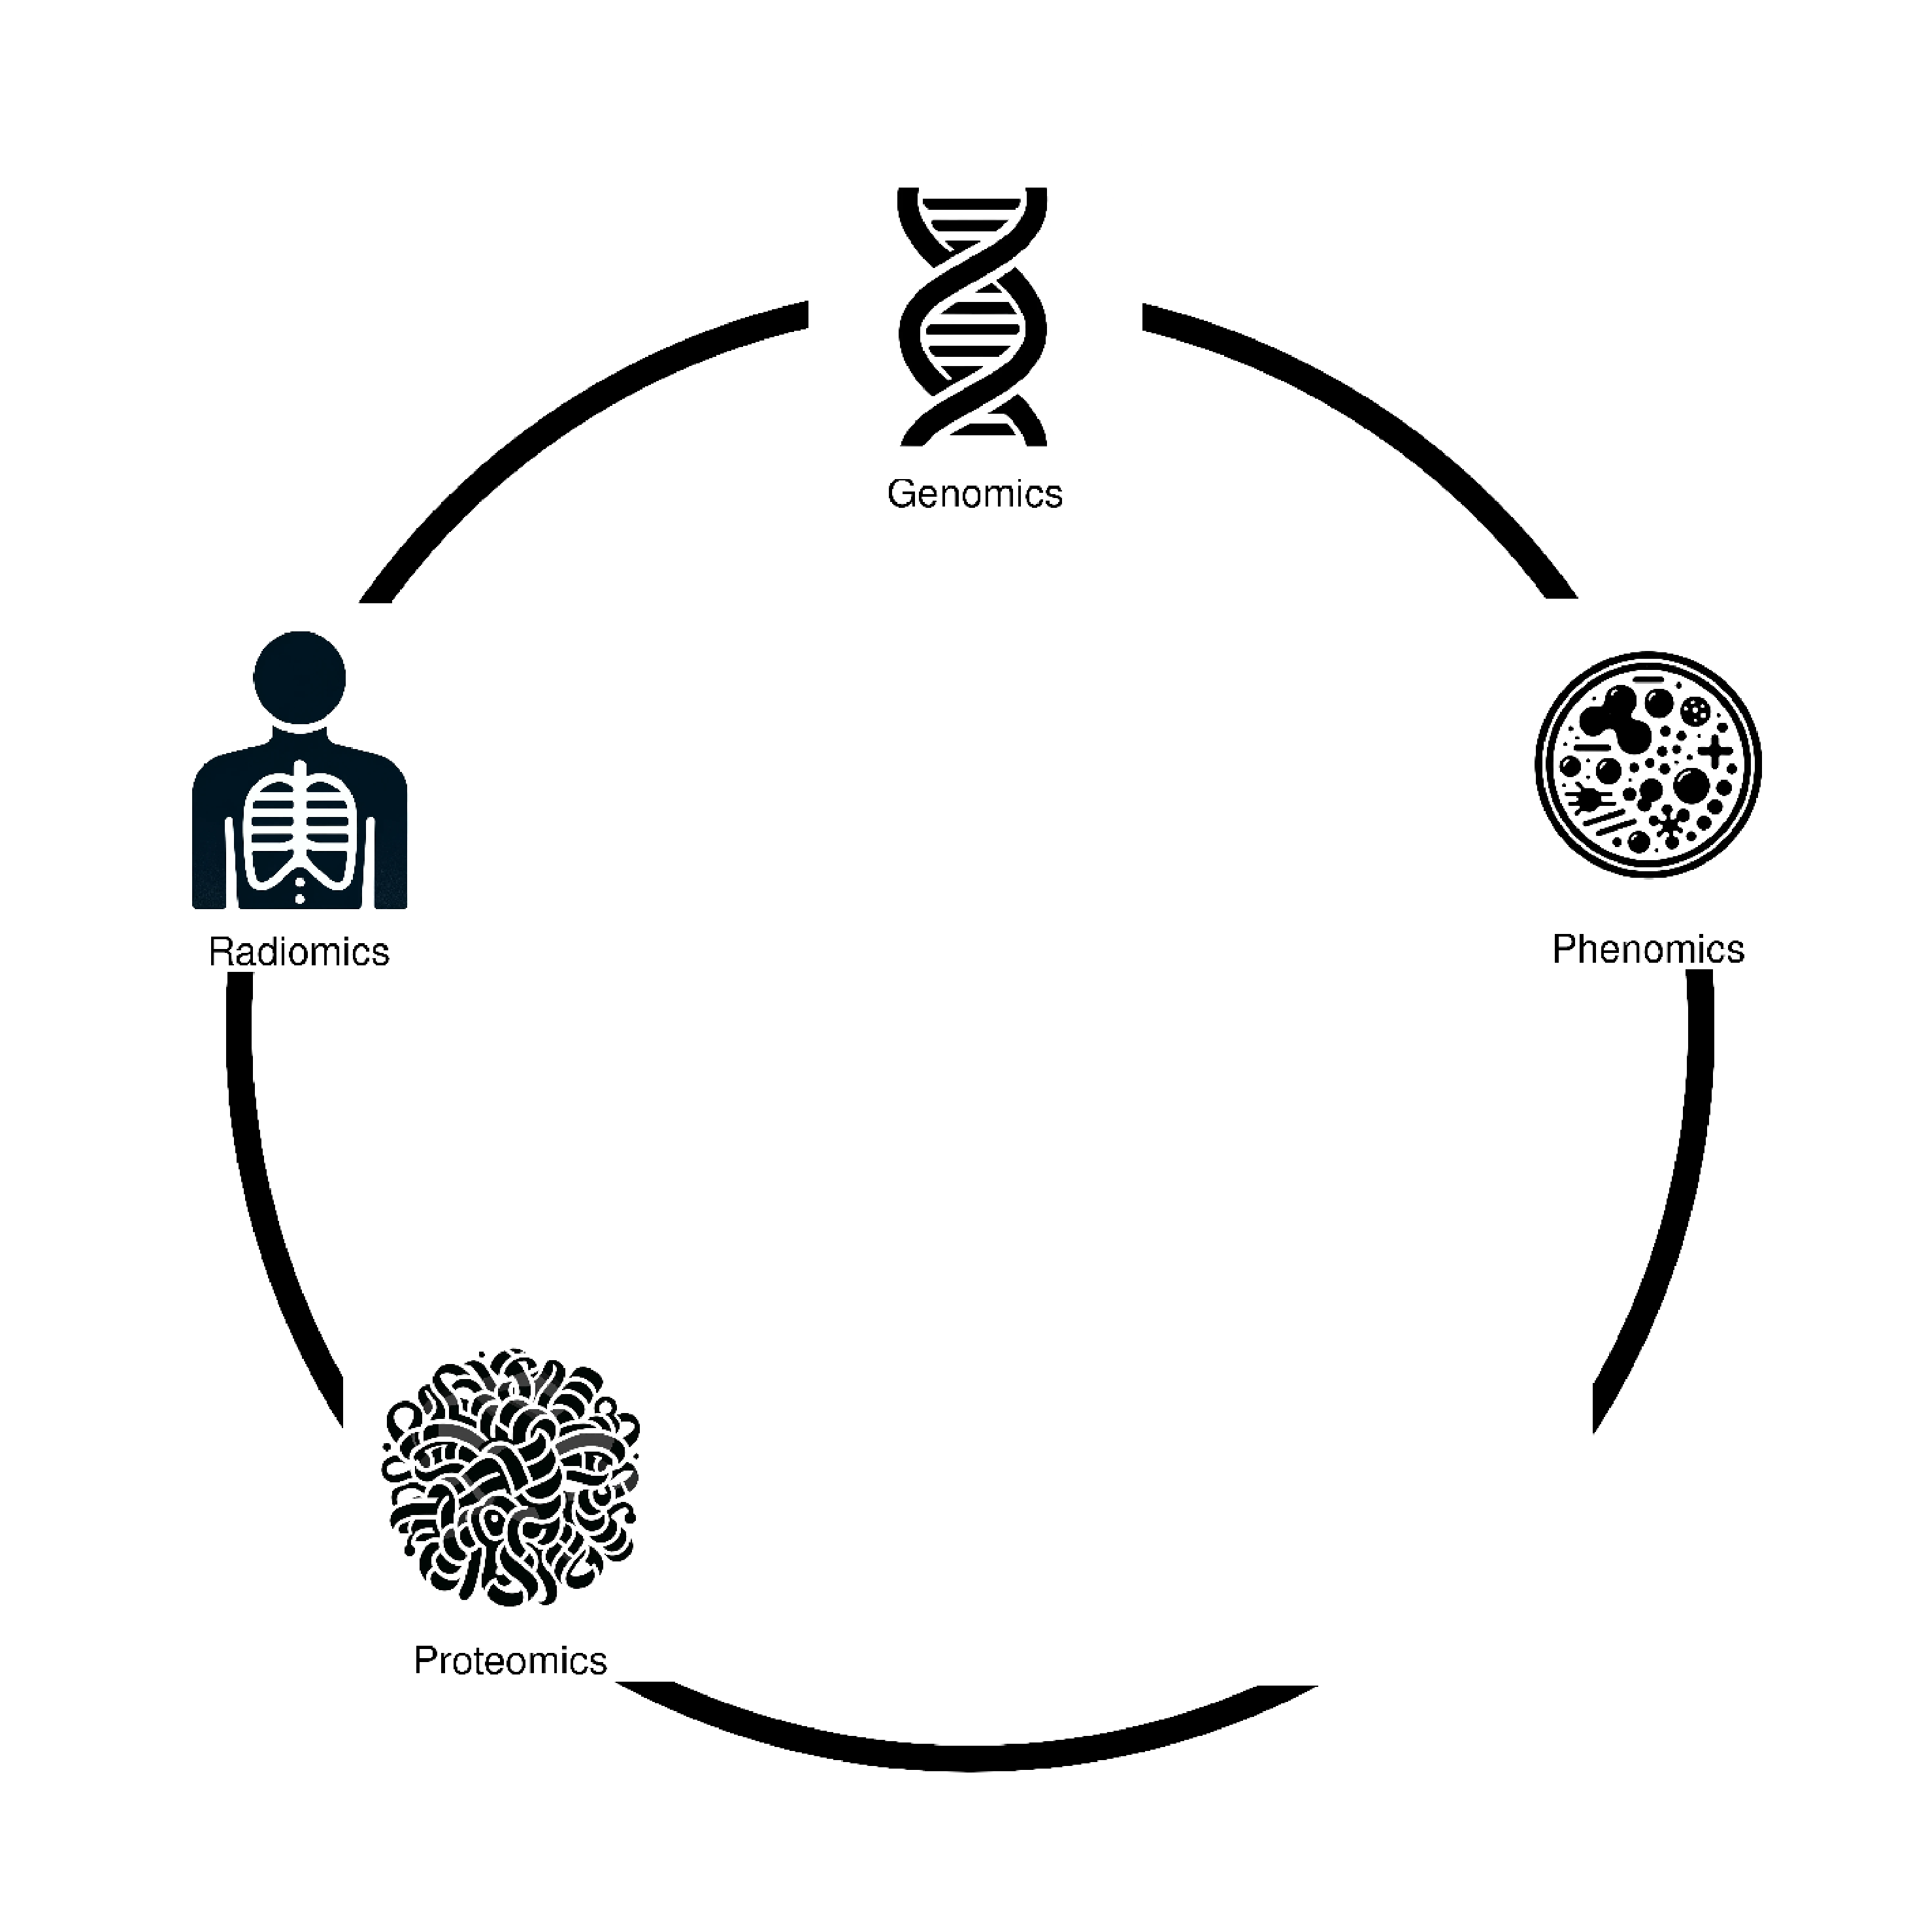
\includegraphics[width=\textwidth]{images/approaches_current.eps}}%
			\only<3-4>{\includegraphics[width=\textwidth]{images/approaches_future.eps}}%
		\end{figure}
	\end{minipage} 
	\begin{minipage}{0.39\textwidth}
		\only<1-2>{\begin{minipage}[t][0.41\paperheight][t]{\textwidth}
			\onslide<1-2>{\begin{block}{Personalised Medicine}
				characterizing a patient and customizing their treatment according to which sub-population they fall into	
		\end{block}}%
		\end{minipage}
		\begin{minipage}[t][0.41\paperheight][t]{\textwidth}
			\onslide<2>{\begin{block}{Biomarkers}
				measurable quantities that can aid in diagnosis and treatment of a disease
		\end{block}}%
\end{minipage}}%
		\only<3-4>{\begin{minipage}[t][0.55\paperheight][t]{\textwidth}
			\onslide<3-4>{\begin{block}{Model Based Approach}
				use patient specific parameters to setup well-defined computational models that output biomarkers which are strongly and causally related to the occurrence or the outcome of a disease
		\end{block}}%
		\end{minipage}
		\begin{minipage}[t][0.27\paperheight][t]{\textwidth}
			\onslide<4>{\begin{block}{Example}
				$\hookrightarrow$
		\end{block}}%
\end{minipage}}%
	\end{minipage}
\end{frame}

\subsection{Example}
\begin{frame}<1-11>[label=ph]
	\frametitle{Example: Pulmonary Hypertension (PH)}
	\begin{itemize}
		\item<1-> affects large parts of the population
		\item<2-> heavily studied but currently no accurate predictive technique
		\item<3-> \begin{tabularx}{\linewidth}{| >{\centering\arraybackslash}m{0.4\linewidth} | >{\centering\arraybackslash}m{0.25\linewidth} | >{\centering\arraybackslash}X |} 
				\hline
				biomarker(s) & measurement & correlation \\ 
				\hline
				\hline
				absolute vascular pressure & \textcolor<4->{red}{micro surgery} & \textcolor<5->{green}{strong} \\ 
				\hline
				brain natriuretic peptide & \textcolor<6->{green}{blood sampling} & \textcolor<7->{red}{weaker} \\ 
				\hline
			\end{tabularx}
		\item<8->
			$\Rightarrow$ accurately determining the absolute vascular pressure through a computational model would allow \textcolor<9->{green}{reliable prognosis} of PH while \textcolor<10->{green}{avoiding the risk} of an invasive procedure
	\end{itemize}
\end{frame}

\section{Model Pipeline}
\subsection{3D Model Pipeline}
\begin{frame}<1-2>[label=mp]
	\only<1-2>{\frametitle{3D Model Pipeline}}
	\only<3>{\frametitle{1D Model Pipeline}}
	\only<4>{\frametitle{3D Geometry Extraction}}
	\only<5>{\frametitle{1D Geometry Extraction}}
	\only<6>{\frametitle{Setting Parameters}}
	\only<7>{\frametitle{Solver}}
	\only<8>{\frametitle{Biomarkers}}
	\only<9->{\frametitle{1D Model Pipeline Recall}}
	\only<100>{\frametitle{Parameter Inference Pipeline}}
	\only<101->{\frametitle{Parameter Inference}}
	\begin{figure}[]%
		\begin{minipage}[t][0.06\paperheight][t]{\linewidth}%
				\only<-99>{\begin{minipage}{0.18\linewidth}%
					\caption*{\tiny Medical Imaging}%
				\end{minipage}%
				\begin{minipage}{0.153\linewidth}%
					\caption*{\tiny}%
				\end{minipage}%
				\begin{minipage}{0.18\linewidth}%
					\caption*{\tiny 3D Geometry}%
				\end{minipage}%
				\begin{minipage}{0.153\linewidth}%
					\caption*{\tiny}%
				\end{minipage}%
				\only<1-2>{\begin{minipage}{0.18\linewidth}%
						\caption*{\tiny}%
				\end{minipage}}%
				\only<3->{\begin{minipage}{0.18\linewidth}%
						\caption*{\tiny 1D Geometry}%
				\end{minipage}}%
				\begin{minipage}{0.153\linewidth}%
					\caption*{\tiny}%
			\end{minipage}}%
		\only<100-101>{
				\begin{minipage}{0.153\linewidth}
					\caption*{\tiny}
				\end{minipage}
				\hfill
				\begin{minipage}{0.58\linewidth}
					\caption*{\tiny Parameter Inference}
				\end{minipage}
				\hfill
				\begin{minipage}{0.153\linewidth}
					\caption*{\tiny }
			\end{minipage}}
		\end{minipage}
		\begin{minipage}[c][0.33\paperheight][c]{\linewidth}%
			\only<-99>{%
				\only<1-3,5-99>{%
					\begin{minipage}{0.18\linewidth}%
						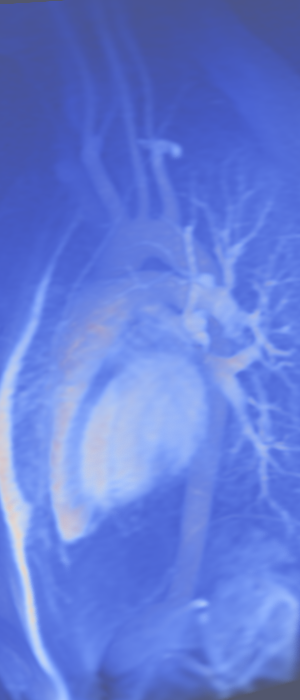
\includegraphics[width=\linewidth]{images/medical_imaging_0007.eps}%
				\end{minipage}%
					\begin{minipage}{0.153\linewidth}%
						\centering
						
\includegraphics[width=0.66\linewidth]{images/right_arrow.png}%
				\end{minipage}}%
				\only<1-3,6-99>{%
					\begin{minipage}{0.18\linewidth}%
						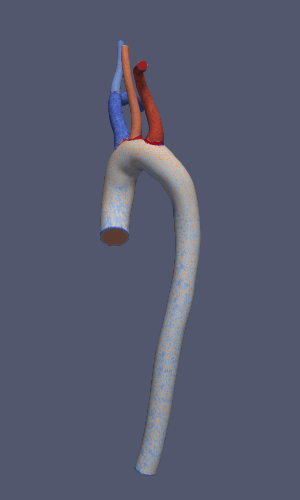
\includegraphics[width=\linewidth]{images/3d_model_0007.eps}%
				\end{minipage}}%
				\only<4>{{\setlength{\fboxsep}{-0.4pt}\fcolorbox{red}{white}{%
							\begin{minipage}{0.18\linewidth}%
								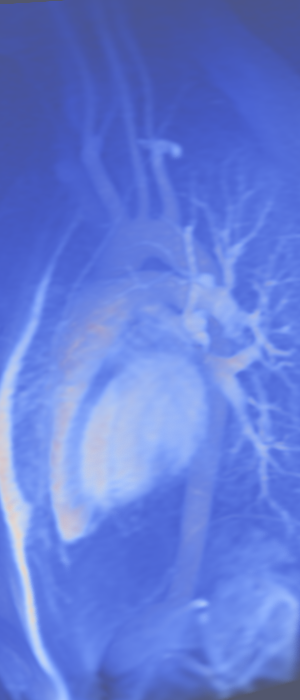
\includegraphics[width=\linewidth]{images/medical_imaging_0007.eps}%
							\end{minipage}%
							\begin{minipage}{0.153\linewidth}%
								\centering
								
\includegraphics[width=0.66\linewidth]{images/right_arrow.png}%
							\end{minipage}%
							\begin{minipage}{0.18\linewidth}%
								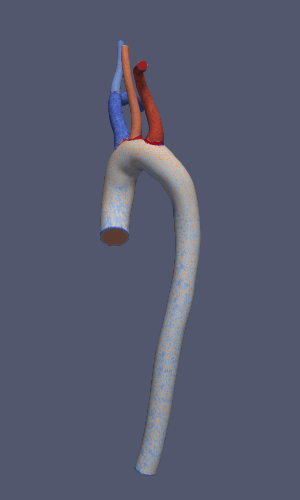
\includegraphics[width=\linewidth]{images/3d_model_0007.eps}%
				\end{minipage}}}}%
				\only<5>{{\setlength{\fboxsep}{-0.4pt}\fcolorbox{red}{white}{%
							\begin{minipage}{0.18\linewidth}%
								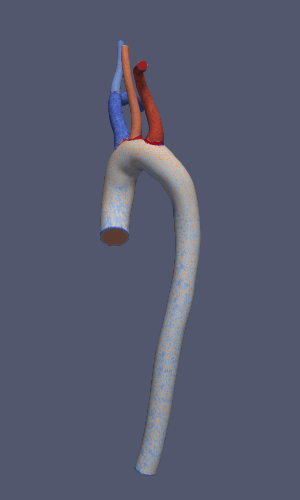
\includegraphics[width=\linewidth]{images/3d_model_0007.eps}%
				\end{minipage}%
				\begin{minipage}{0.153\linewidth}%
					\centering
					
\includegraphics[width=0.66\linewidth]{images/right_arrow.png}%
				\end{minipage}%
				\only<1-2>{\begin{minipage}{0.18\linewidth}%
						{\huge .\hfill .\hfill .}%
				\end{minipage}}%
				\only<3->{\begin{minipage}{0.18\linewidth}%
						\includegraphics[width=\linewidth]{images/1d_model_0007.eps}%
				\end{minipage}}%
	}}}%
				\only<1-4,6-99>{%
				\begin{minipage}{0.153\linewidth}%
					\centering
					
\includegraphics[width=0.66\linewidth]{images/right_arrow.png}%
				\end{minipage}%
				\only<1-2>{\begin{minipage}{0.18\linewidth}%
						{\huge .\hfill .\hfill .}%
				\end{minipage}}%
				\only<3->{\begin{minipage}{0.18\linewidth}%
						\includegraphics[width=\linewidth]{images/1d_model_0007.eps}%
			\end{minipage}}}%
				\begin{minipage}{0.153\linewidth}%
					\centering
					
\includegraphics[width=0.66\linewidth]{images/right_arrow.png}%
			\end{minipage}}%
			\only<100-101>{%
				\begin{minipage}{0.027\linewidth}%
					\caption*{\tiny}
				\end{minipage}%
				\begin{minipage}{0.153\linewidth}%
					\centering
					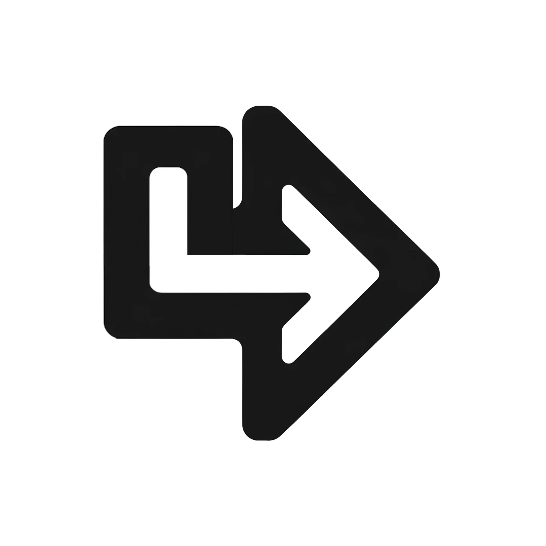
\includegraphics[angle=270, width=0.66\linewidth]{images/left_turn_arrow.eps}%
				\end{minipage}%
				\only<100>{\begin{minipage}{0.663\linewidth}%
					{\footnotesize \begin{itemize} %
							\item MCMC \& gradient information $\rightarrow$ Hamiltionian Monte Carlo (HMC)%
							\item HMC \& adaptively setting path length $\rightarrow$ No-U-Turn Sampler (NUTS)%
							\item Provided by Numpyro%
					\end{itemize}}%
			\end{minipage}}%
				\only<101>{{\setlength{\fboxsep}{-0.4pt}\fcolorbox{red}{white}{\begin{minipage}{0.663\linewidth}%
					{\footnotesize \begin{itemize} %
							\item MCMC \& gradient information $\rightarrow$ Hamiltionian Monte Carlo (HMC)%
							\item HMC \& adaptively setting path length $\rightarrow$ No-U-Turn Sampler (NUTS)%
							\item Provided by Numpyro%
					\end{itemize}}%
	\end{minipage}}}}%
				\begin{minipage}{0.153\linewidth}%
					\centering
					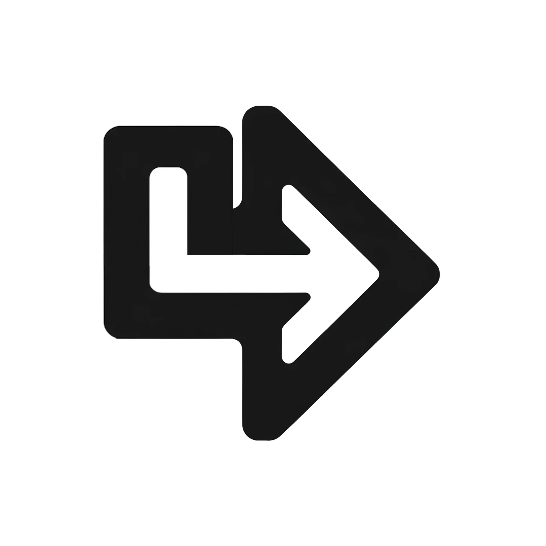
\includegraphics[angle=180, width=0.66\linewidth]{images/left_turn_arrow.eps}%
			\end{minipage}}%
		\end{minipage}%
		\vfill%
		\begin{minipage}[t][0.06\paperheight][t]{\linewidth}%
			\begin{minipage}{0.18\linewidth}%
				\caption*{\tiny Parameters}%
			\end{minipage}%
			\begin{minipage}{0.153\linewidth}%
				\caption*{\tiny}%
			\end{minipage}%
			\begin{minipage}{0.18\linewidth}%
				\caption*{\tiny Solver}%
			\end{minipage}%
			\begin{minipage}{0.153\linewidth}%
				\caption*{\tiny}%
			\end{minipage}%
			\begin{minipage}{0.18\linewidth}%
				\caption*{\tiny Biomarkers}%
			\end{minipage}%
			\begin{minipage}{0.153\linewidth}%
				\caption*{\tiny}%
			\end{minipage}%
		\end{minipage}
		\begin{minipage}[c][0.33\paperheight][c]{\linewidth}%
			\begin{minipage}{0.18\linewidth}%
				\includegraphics<1-2>[width=\linewidth]{images/bifurcation_3D.eps}%
				\includegraphics<3-5,7->[width=\linewidth]{images/bifurcation_1D.eps}%
				\only<6>{{\setlength{\fboxsep}{-0.4pt}\fcolorbox{red}{white}{%
				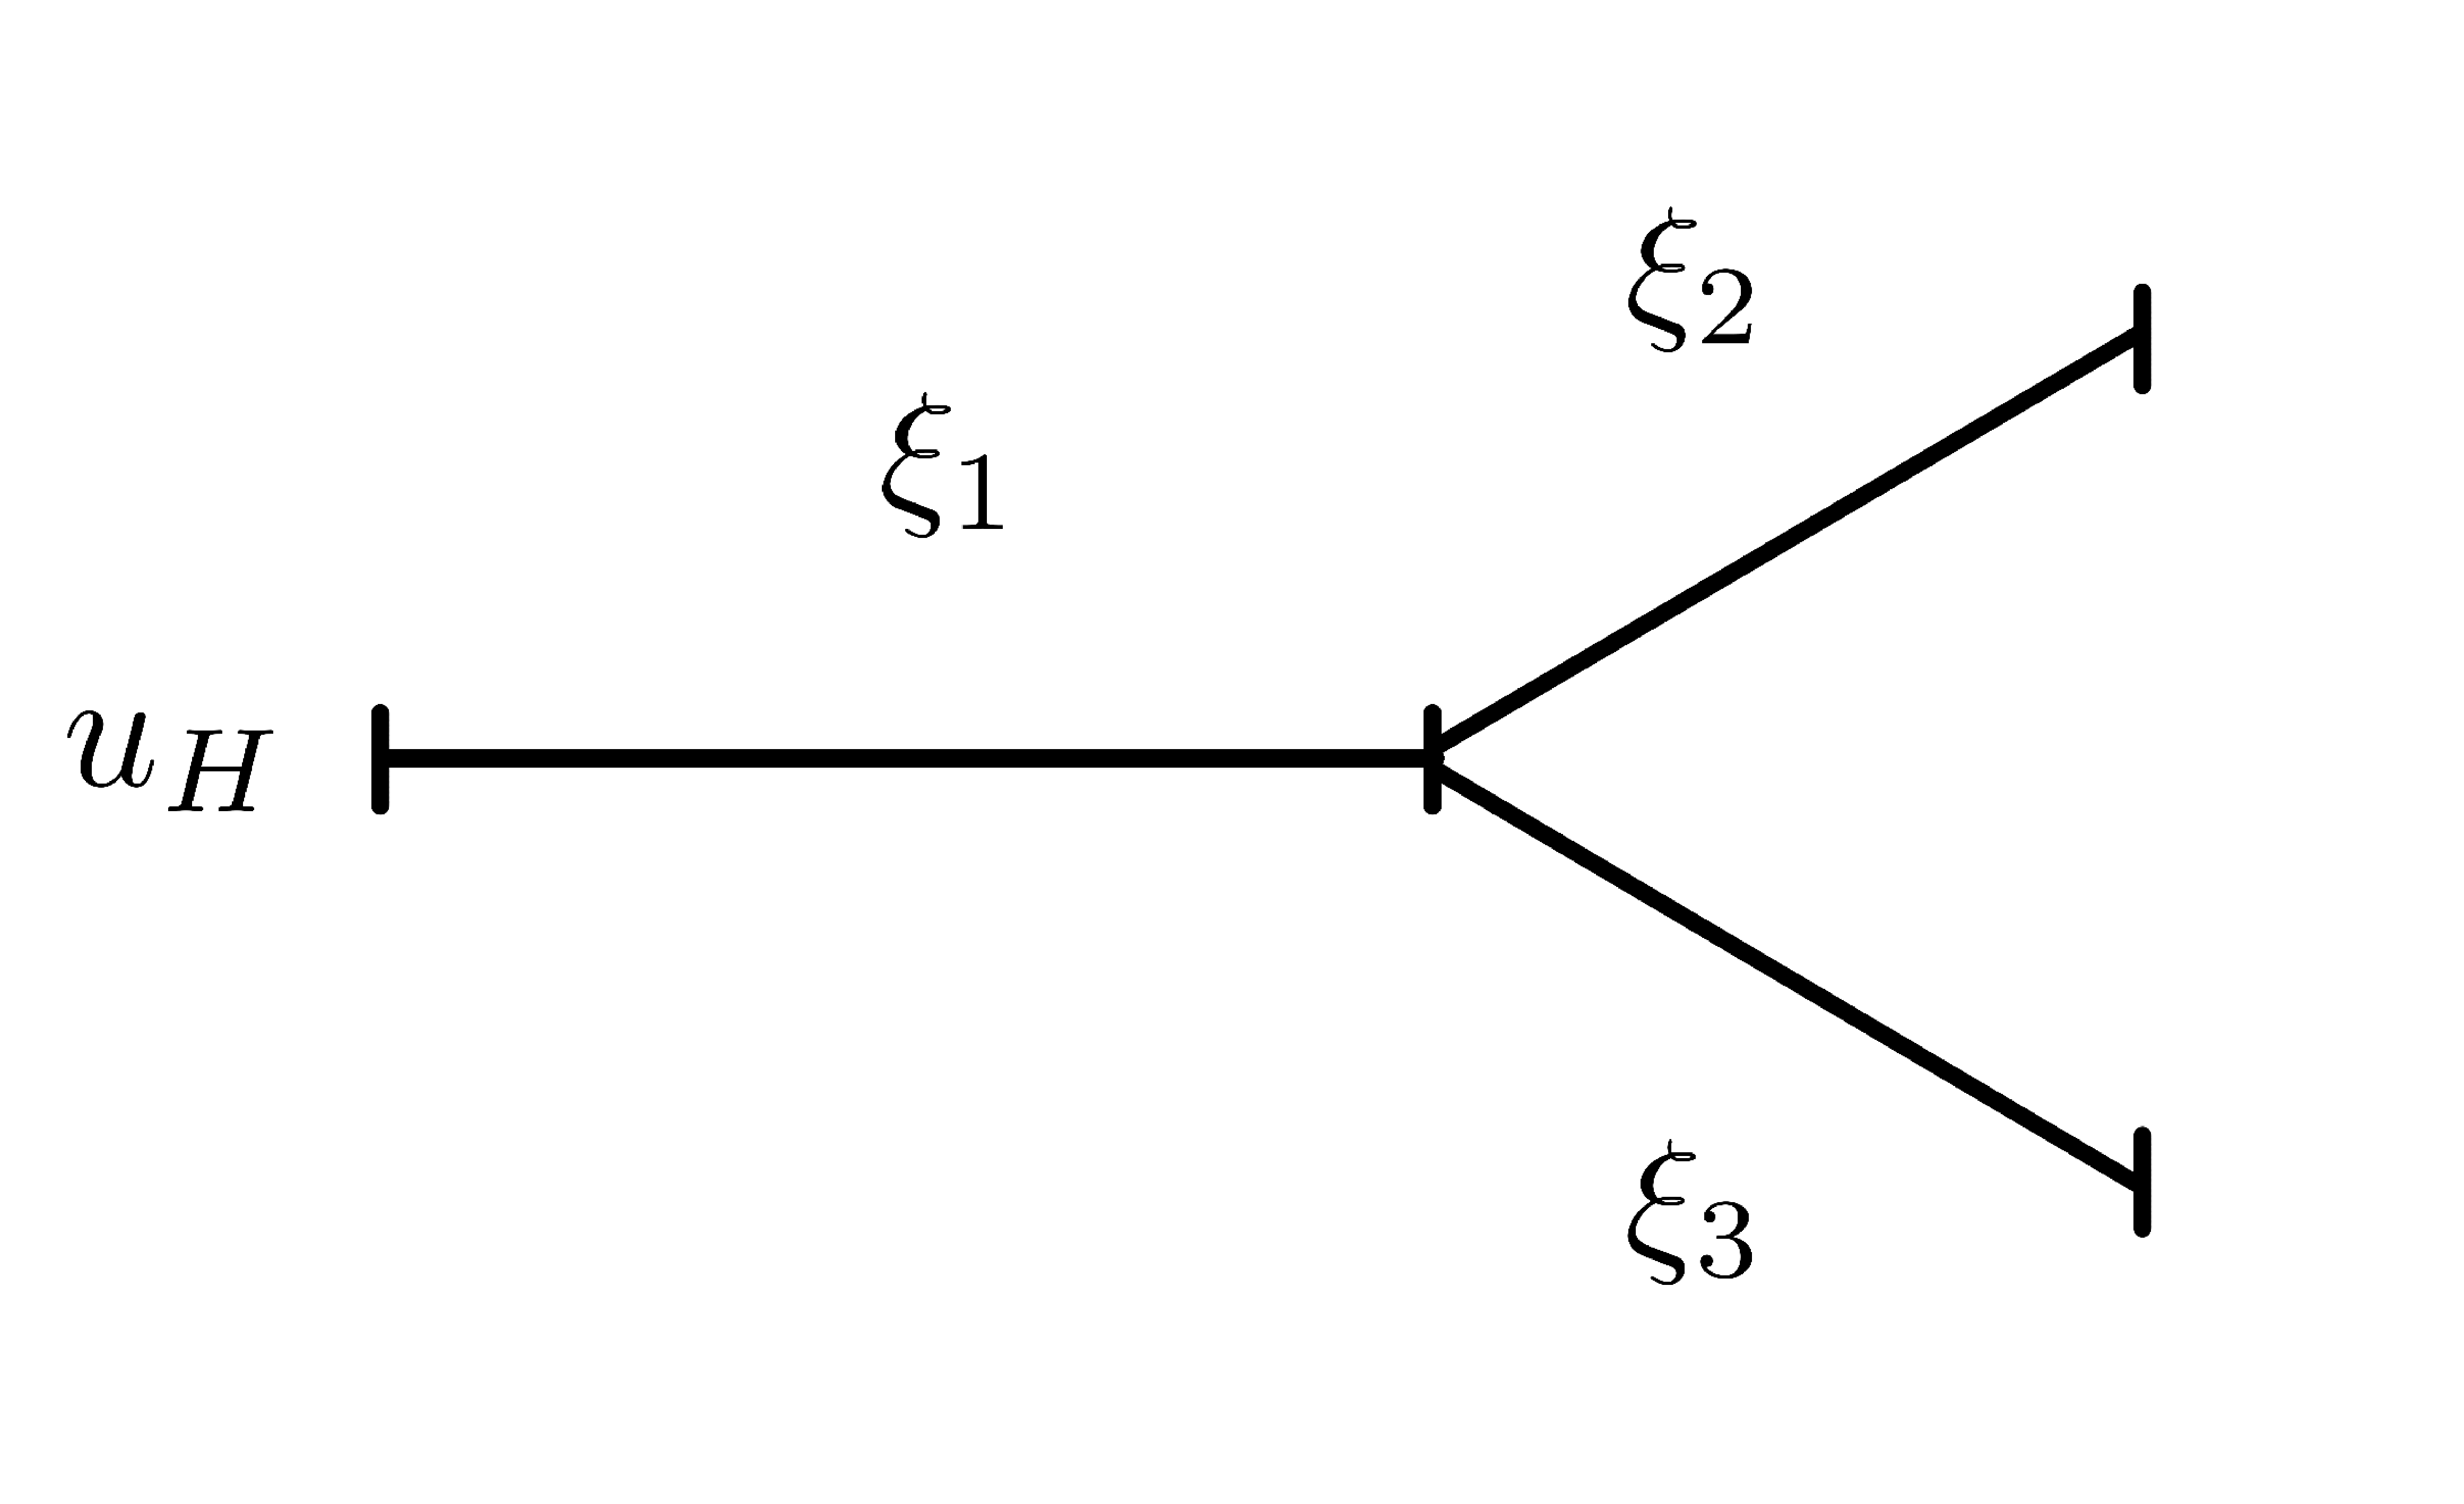
\includegraphics[width=\linewidth]{images/bifurcation_1D.eps}}}}%
			\end{minipage}%
			\begin{minipage}{0.153\linewidth}%
				\centering
				
\includegraphics[width=0.66\linewidth]{images/right_arrow.png}%
			\end{minipage}%
			\only<1-2>{\begin{minipage}{0.18\linewidth}%
					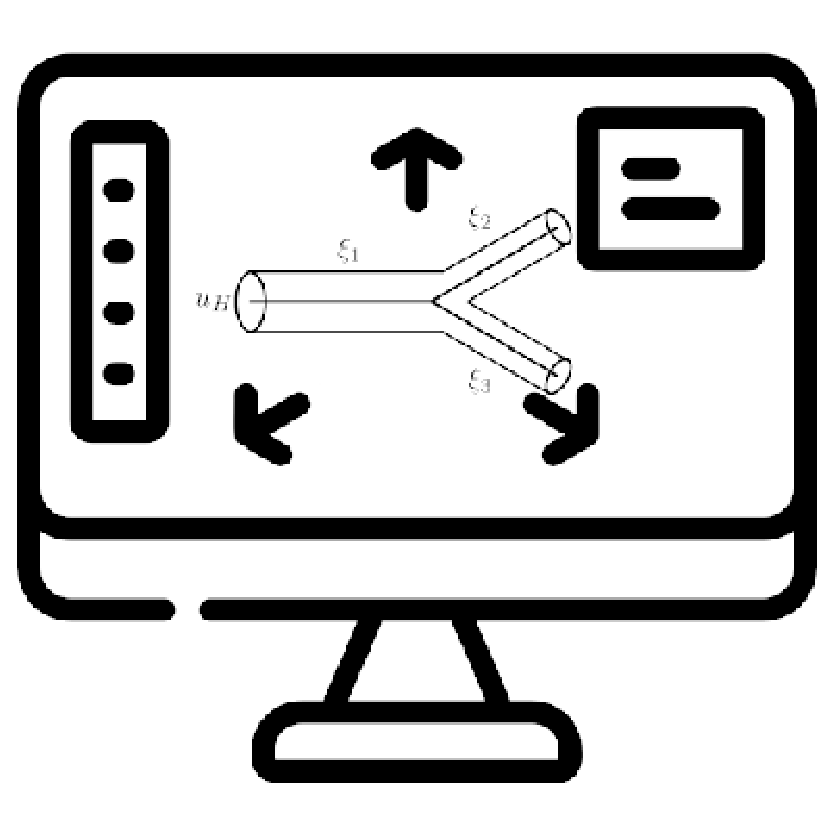
\includegraphics[width=\linewidth]{images/solver_3D.eps}%
			\end{minipage}}%%
			\only<3-6,8->{\begin{minipage}{0.18\linewidth}%
					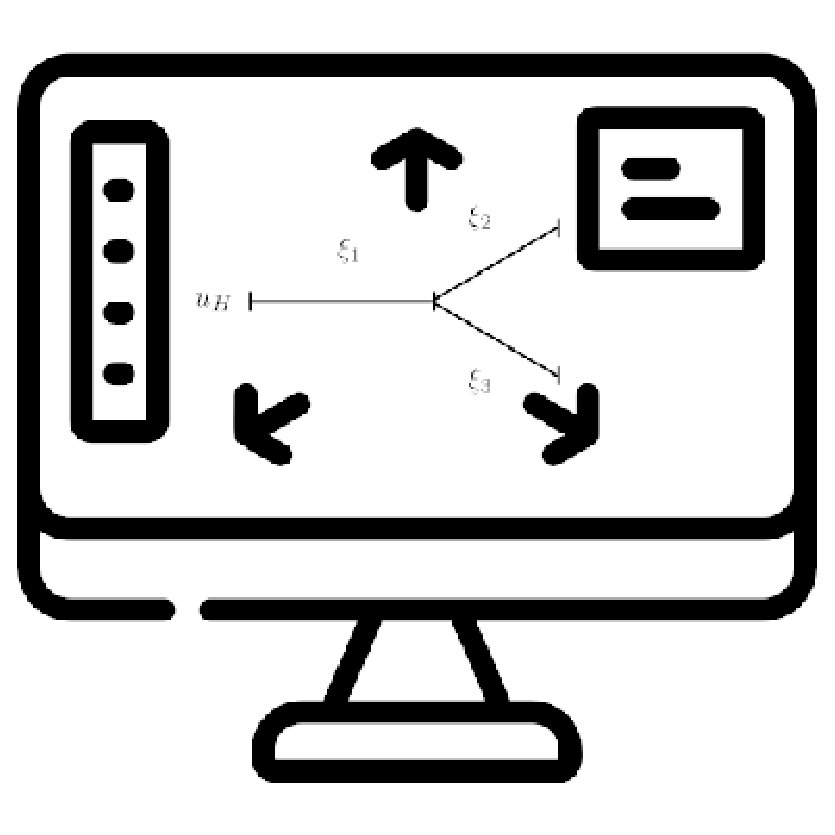
\includegraphics[width=\linewidth]{images/solver_1D.eps}%
			\end{minipage}}%
			\only<7>{{\setlength{\fboxsep}{-0.4pt}\fcolorbox{red}{white}{\begin{minipage}{0.18\linewidth}%
					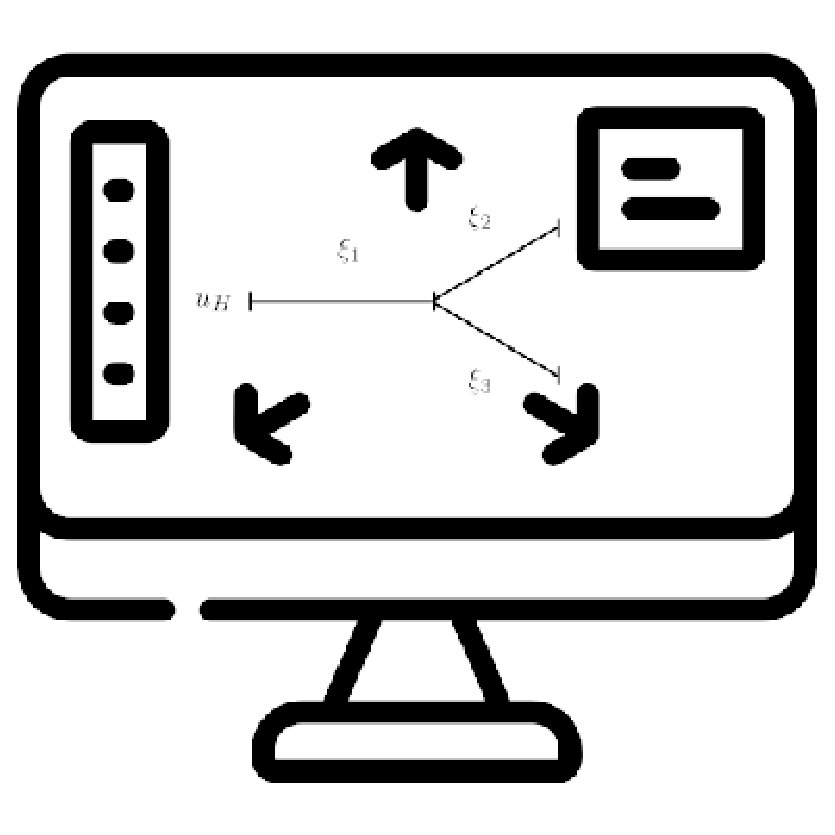
\includegraphics[width=\linewidth]{images/solver_1D.eps}%
	\end{minipage}}}}%
			\begin{minipage}{0.153\linewidth}%
				\centering
				
\includegraphics[width=0.66\linewidth]{images/right_arrow.png}%
			\end{minipage}%
			\only<1-2>{\begin{minipage}{0.18\linewidth}%
					\includegraphics[width=\linewidth]{images/3d_biomarkers_0007.eps}%
			\end{minipage}}%
			\only<3-7,9->{\begin{minipage}{0.18\linewidth}%
					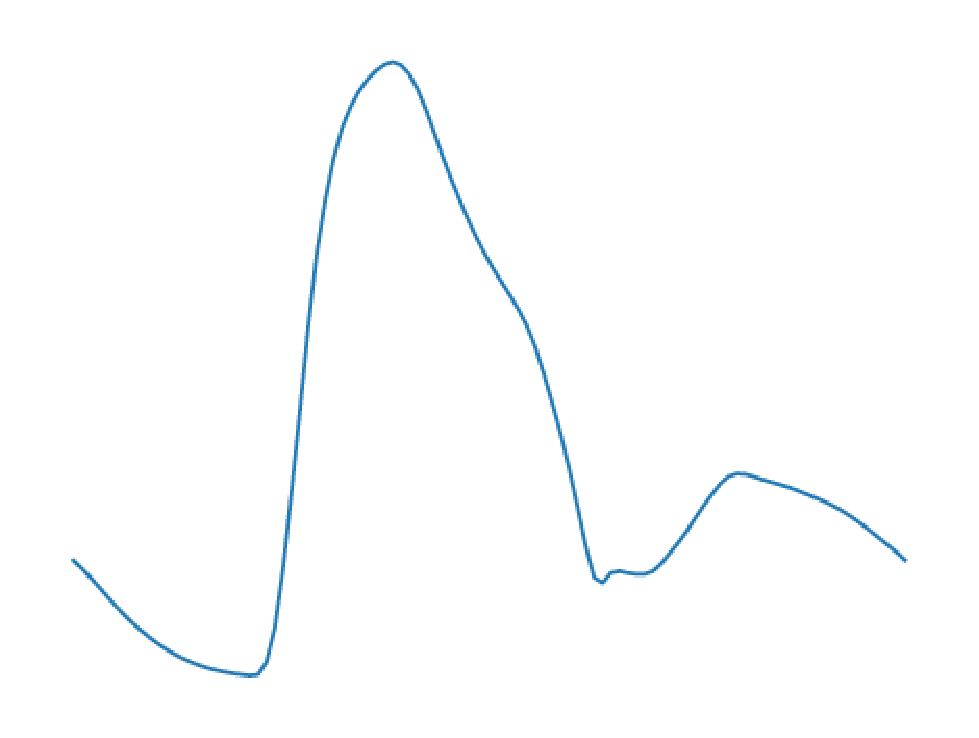
\includegraphics[width=\linewidth]{images/adan56_tibiofibular_trunk_L_P.eps}%
			\end{minipage}}%
			\only<8>{{\setlength{\fboxsep}{-0.4pt}\fcolorbox{red}{white}{\begin{minipage}{0.18\linewidth}%
					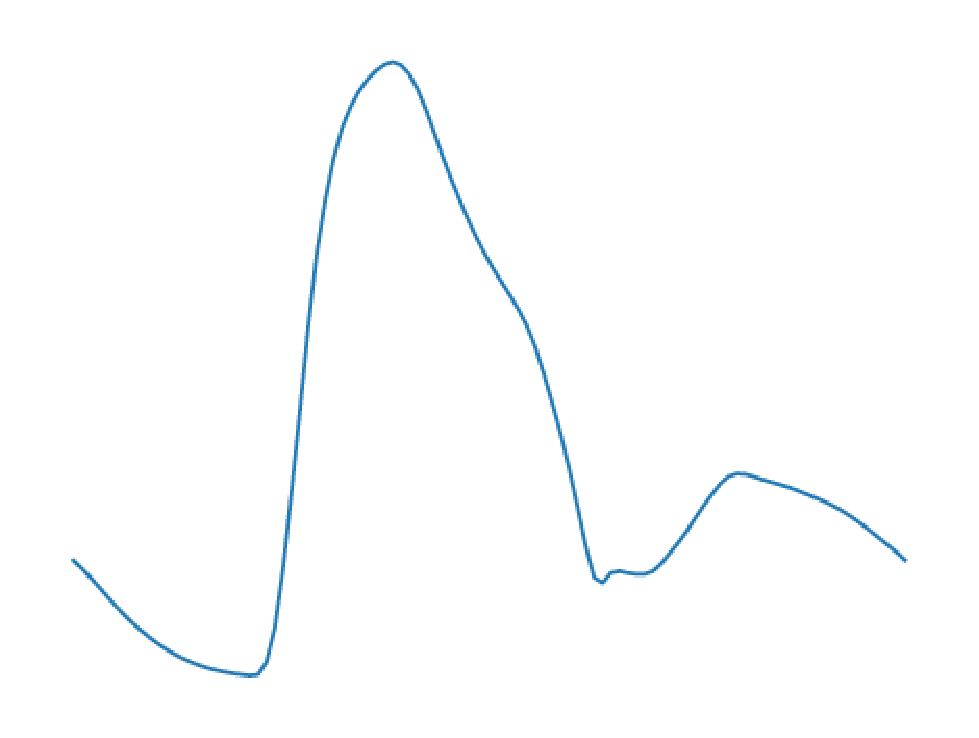
\includegraphics[width=\linewidth]{images/adan56_tibiofibular_trunk_L_P.eps}%
	\end{minipage}}}}%
			\begin{minipage}{0.153\linewidth}%
				\only<1-99>{\caption*{\tiny }}%
				\only<2>{\caption*{\tiny \color{red} too expensive!}}%
				\only<3-99>{\caption*{\tiny }}%
				\centering
				\only<100->{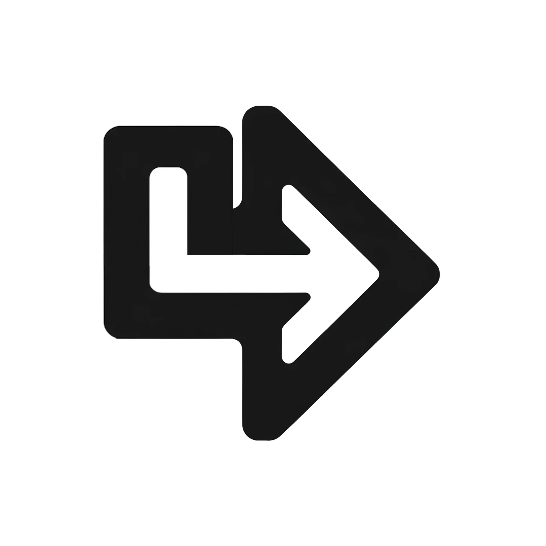
\includegraphics[angle=90, width=0.66\linewidth]{images/left_turn_arrow.eps}}%
			\end{minipage}%
		\end{minipage}%
	\end{figure}%
\end{frame}

\subsection{1D Model Pipeline}
\againframe<3>{mp}
\subsection{3D Geometry Extraction}
\againframe<4>{mp}
\subsection{1D Geometry Extraction}
\againframe<5>{mp}

\subsection{1D Geometry Extraction}
\begin{frame}<1-4>[label=1dge]
	\frametitle{1D Geometry Extraction: Slicer 3D + VMTK}
	\begin{minipage}{\linewidth}
		\onslide<1->{\begin{minipage}{0.25\linewidth}
				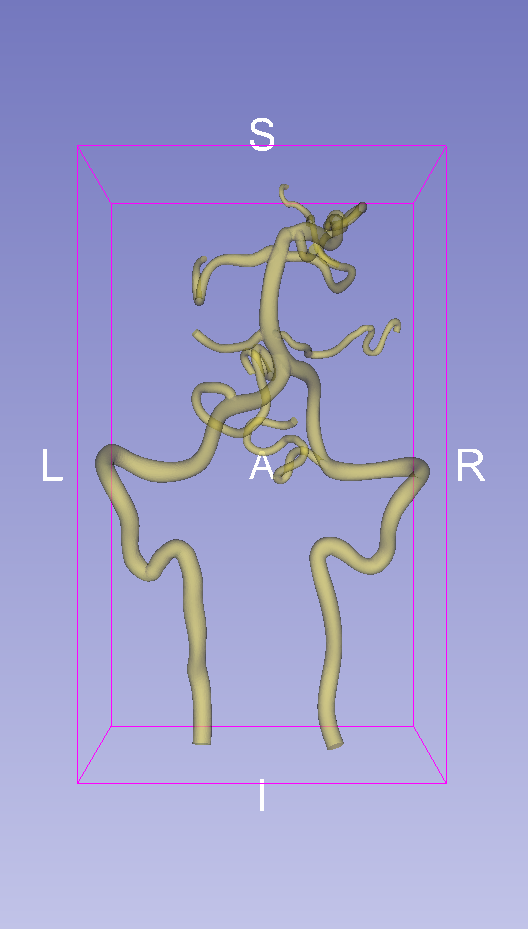
\includegraphics[width=\linewidth]{images/0053_extract1.png}
		\end{minipage}}
		\onslide<3->{\begin{minipage}{0.1\linewidth}
				\scalebox{-1}[1]{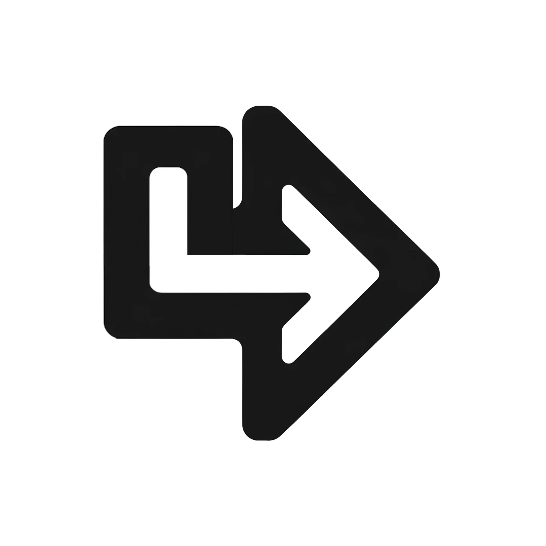
\includegraphics[width=\linewidth, angle=180]{images/left_turn_arrow.eps}}
			\end{minipage}
			\begin{minipage}{0.25\linewidth}
				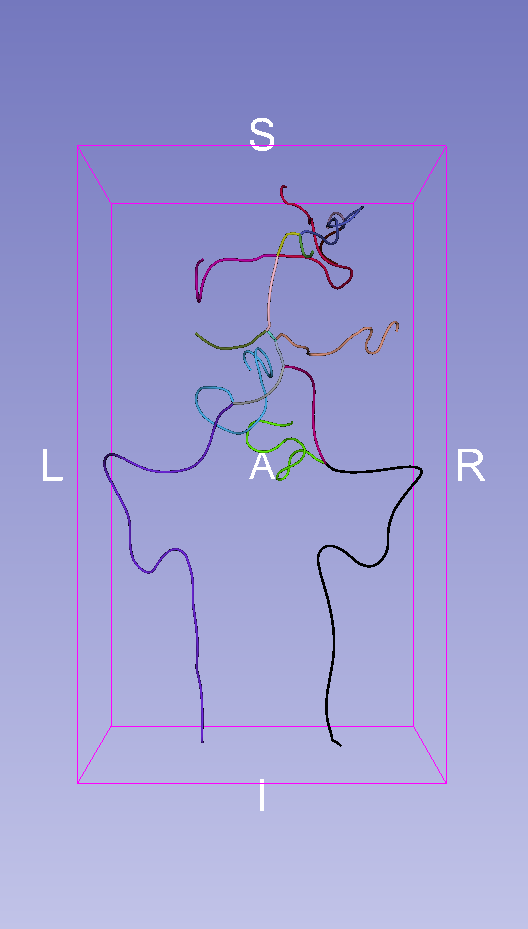
\includegraphics[width=\linewidth]{images/0053_extract3.png}
		\end{minipage}}
		\begin{minipage}{0.37\linewidth}
			{\small \begin{enumerate}
					\item<1-> load meshdata from \emph{vascularmodel.com} in Slicer 3D
					\item<2-> use VMTK plugin to determine start/end points
					\item<3-> extract 1D geometry
					\item<4-> save extracted geometry in table
			\end{enumerate}}
		\end{minipage}
	\end{minipage}
	\begin{minipage}{\linewidth}
		\begin{minipage}{0.075\linewidth}
			{\ }
		\end{minipage}
		\onslide<2->{\begin{minipage}{0.1\linewidth}
				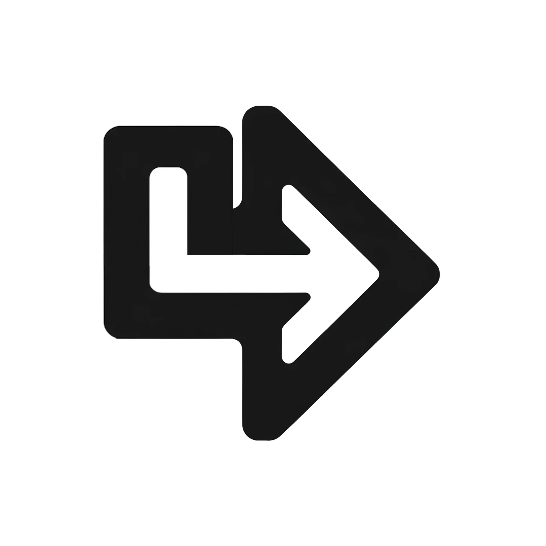
\includegraphics[width=\linewidth]{images/left_turn_arrow.eps}
			\end{minipage}
			\begin{minipage}{0.25\linewidth}
				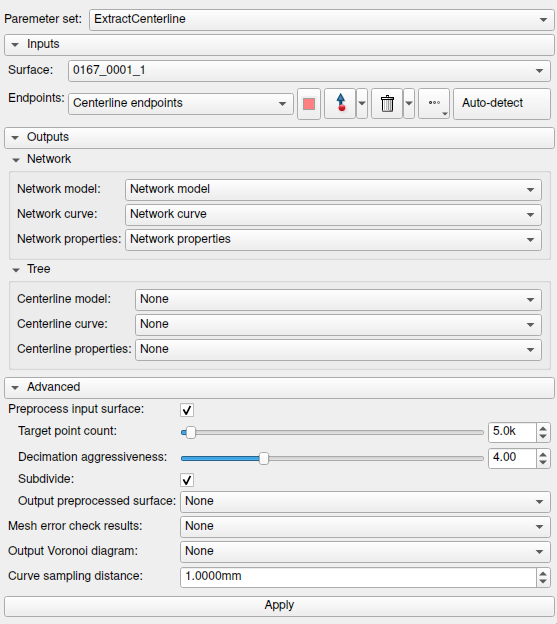
\includegraphics[width=\linewidth]{images/0053_extract2.png}
		\end{minipage}}
		\onslide<4->{\begin{minipage}{0.1\linewidth}
				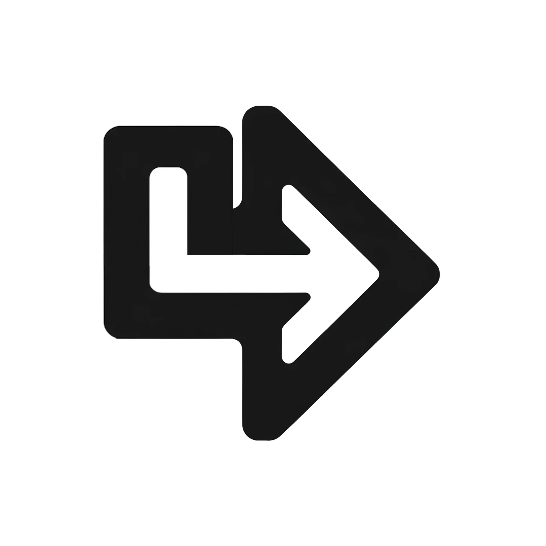
\includegraphics[width=\linewidth]{images/left_turn_arrow.eps}
			\end{minipage}
			\begin{minipage}{0.25\linewidth}
				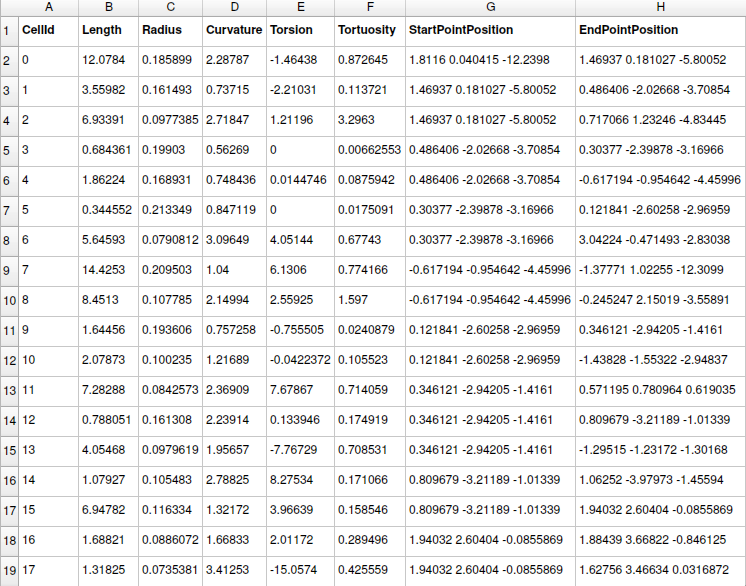
\includegraphics[width=\linewidth]{images/0053_extract4.png}
		\end{minipage}}
		\begin{minipage}{0.195\linewidth}
		\end{minipage}
	\end{minipage}
\end{frame}

\subsection{Setting Parameters}
\againframe<6>{mp}

\begin{frame}<1-3>[label=eb]
	\frametitle{Setting Parameters: Bifurcation Example}
	\begin{figure}
		\begin{center}
			\begin{minipage}[t][0.33\paperheight][t]{\textwidth}
				\begin{minipage}{0.44\textwidth}
					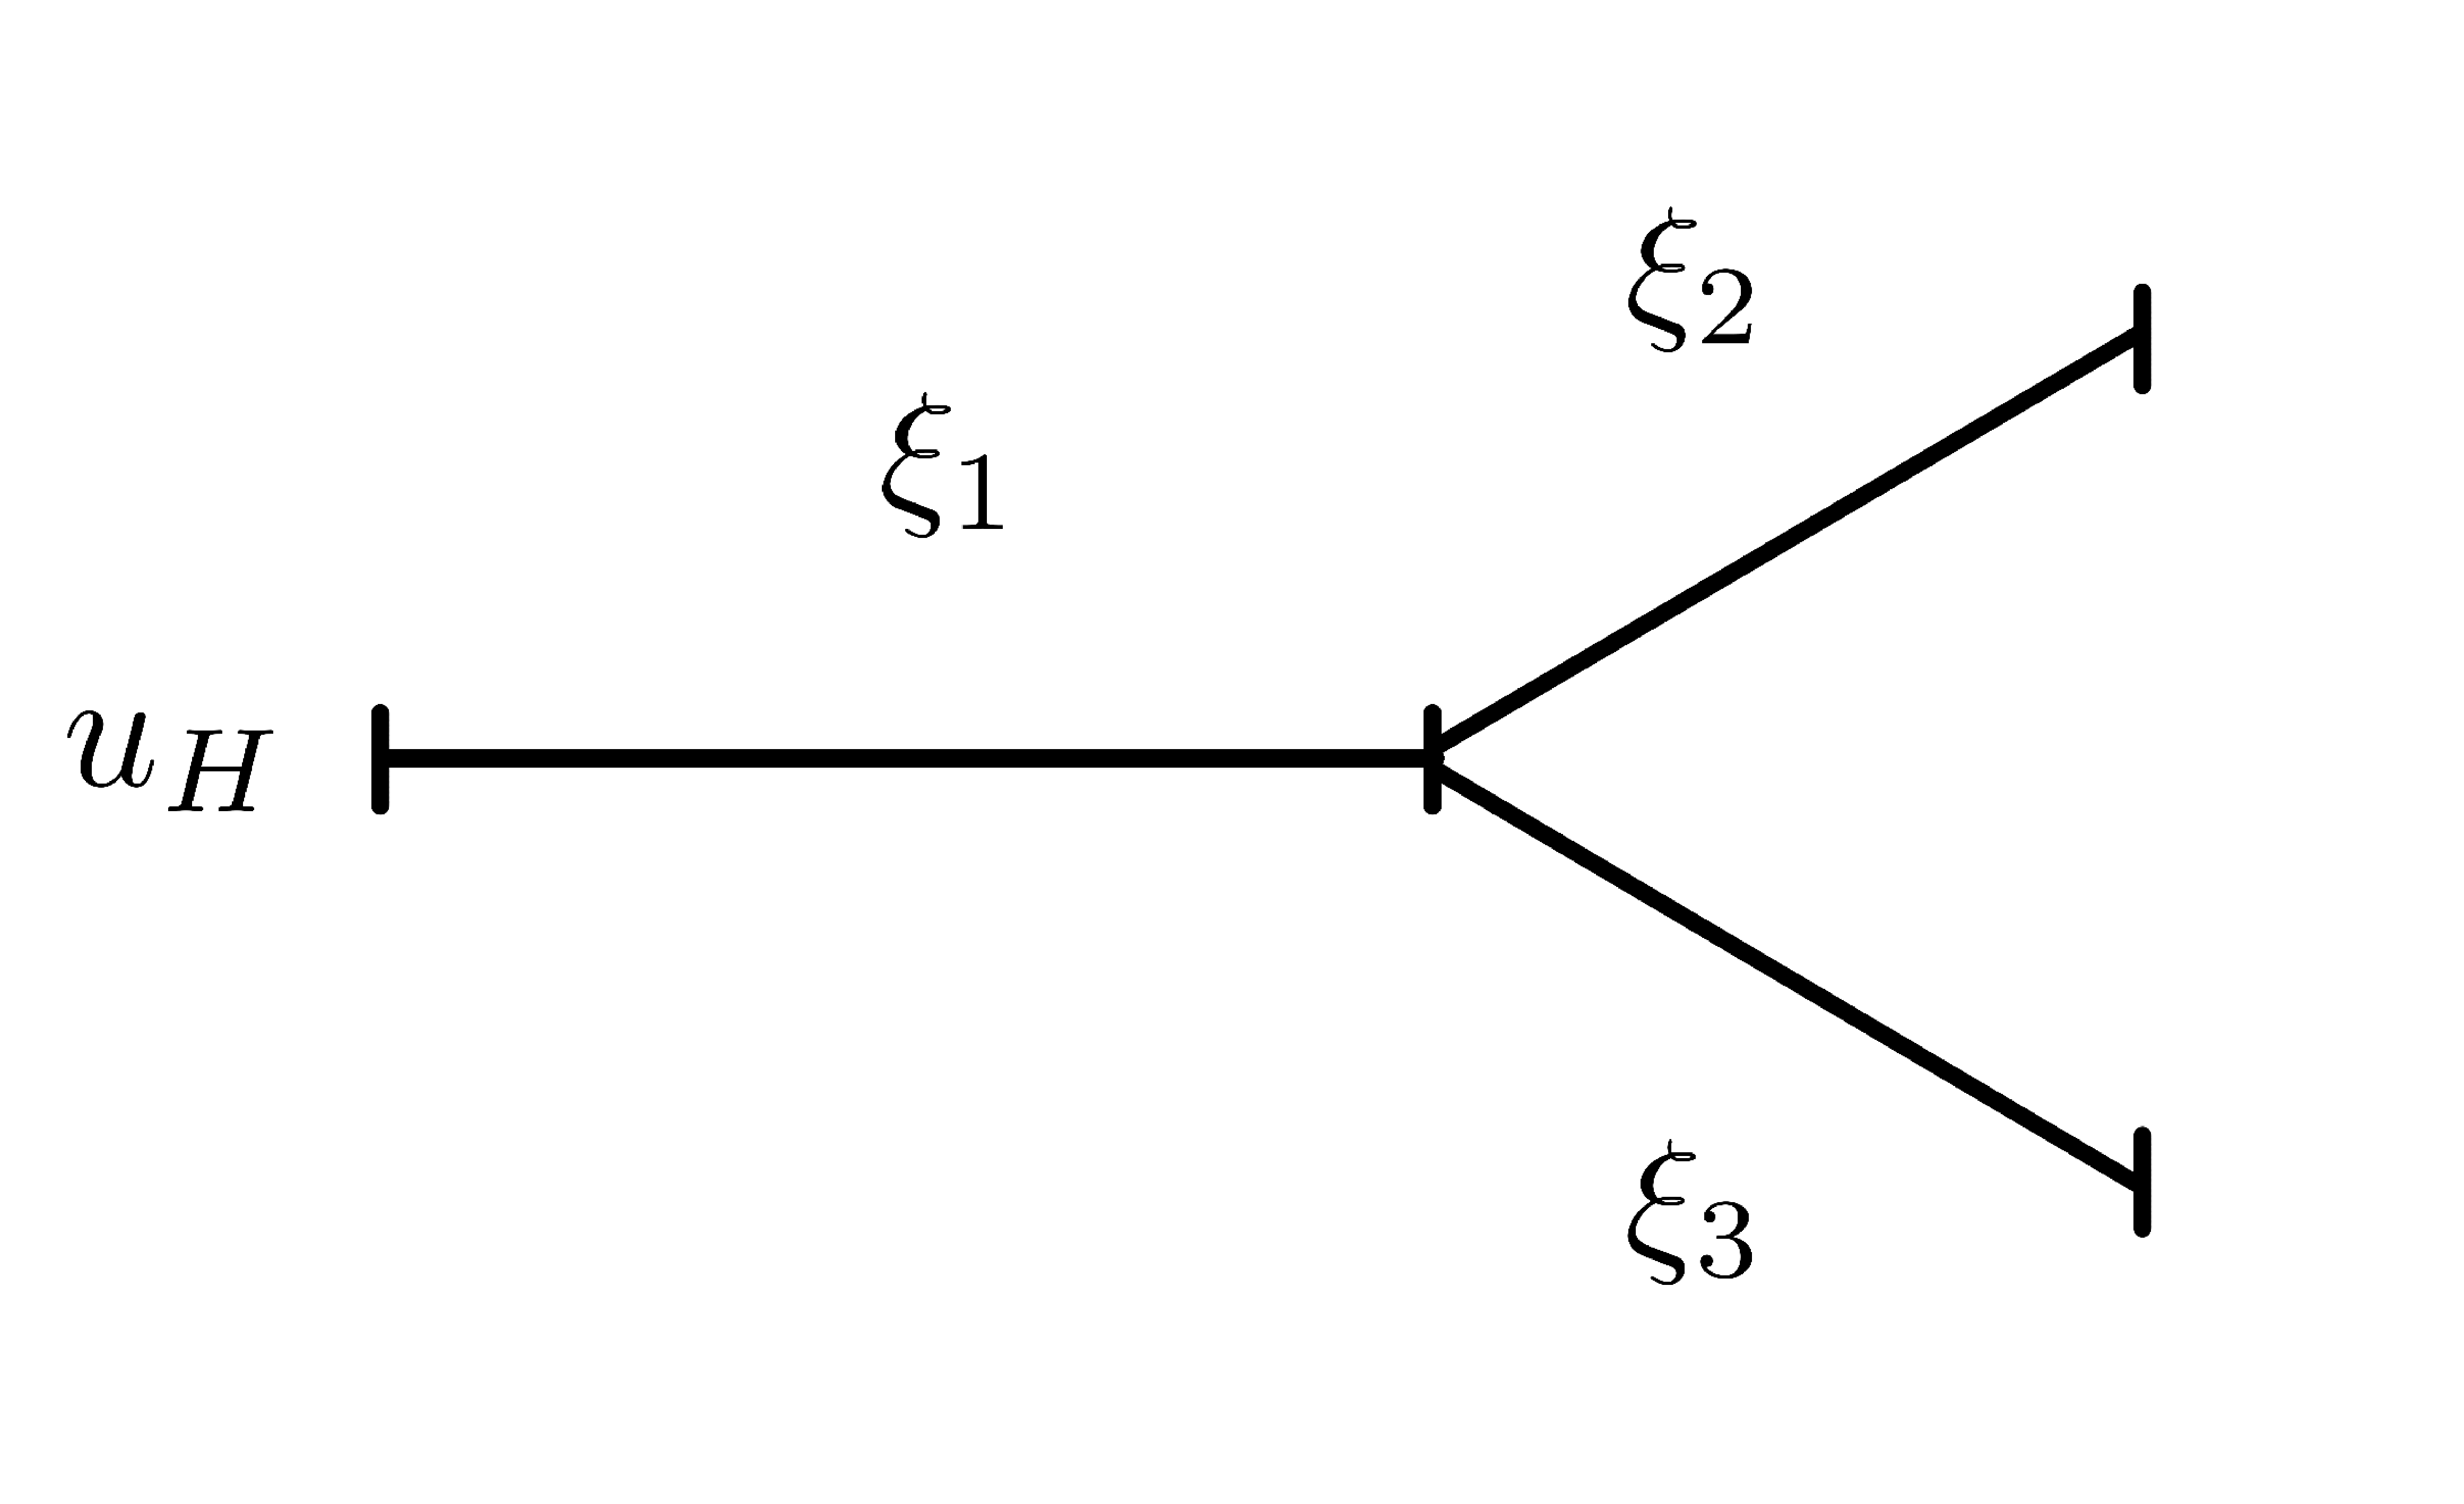
\includegraphics[width=\textwidth]{images/bifurcation_1D.eps}
				\end{minipage}
				\onslide<2->{
					\begin{minipage}{0.09\textwidth}
						
\includegraphics[width=\textwidth]{images/right_arrow.png}
					\end{minipage}
					\begin{minipage}{0.44\textwidth}
						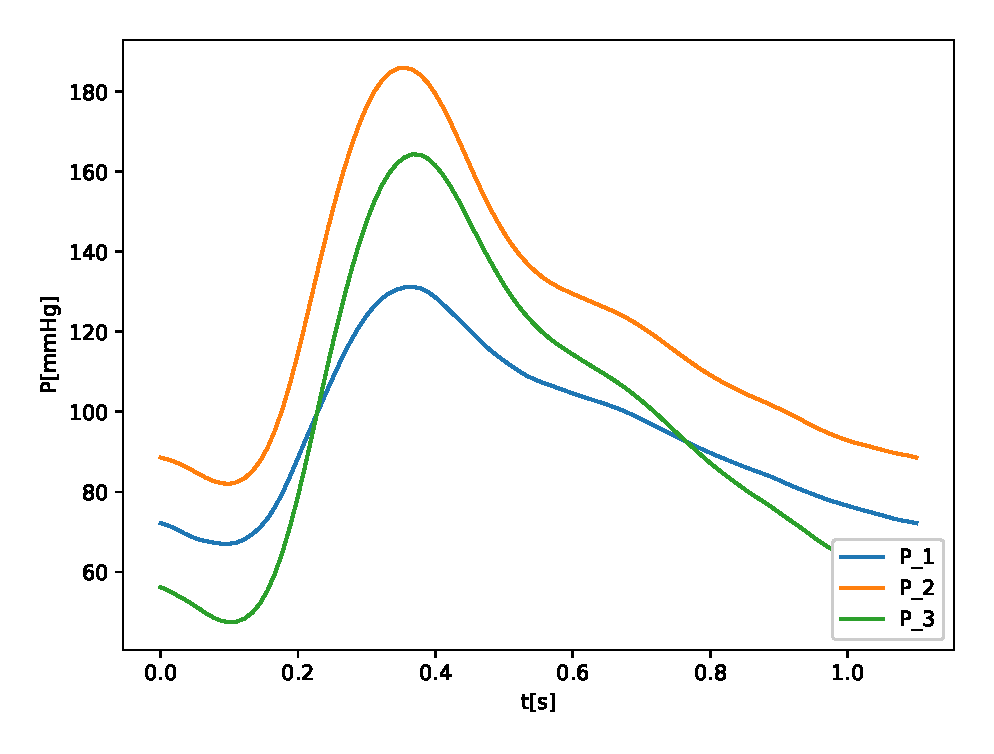
\includegraphics[width=\textwidth]{images/compare_output_params_P_P.eps}
				\end{minipage}}
			\end{minipage}
		\end{center}
	\end{figure}
	\begin{figure}
		\begin{center}
			\only<1-2>{\begin{minipage}[t][0.33\paperheight][t]{\textwidth}
					\begin{minipage}{0.44\textwidth}
						\caption*{The bifurcation $\xi := \{u_H, \xi_1, \xi_2, \xi_3\}$ consists of a driving flow $u_H$ and three vessels: $\xi_1 := \{l^1, h_0^1, A_0^1, E^1\}$, $\xi_2 := \{l^2, h_0^2, A_0^2, E^2, R_1^2, C^2, R_2^2\}$, $\xi_3 := \{l^3, h_0^3, A_0^3, E^3, R_1^3, C^3, R_2^3\}.$}
					\end{minipage}
					\hfill
					\only<2>{\begin{minipage}{0.44\textwidth}
							\caption*{Altering the Windkessel parameters $(R_1,C,R_2)$ leads to vastly different pressure waves being simulated.}
					\end{minipage}}
			\end{minipage}}
		\end{center}
	\end{figure}
	\vspace{-6.36584pt}
	\only<1-2>{
		\begin{minipage}[t][0.1\paperheight][t]{\textwidth}
			{\tiny \centering 
				$u_H \hat{=}$ flow from heart,

				$l \hat{=}$ vessel length,
				$h_0 \hat{=}$ reference vessel wall thickness,
				$A_0 \hat{=}$ reference cross-section,

				$E \hat{=}$ Young's modulus,
				$R_1, C, R_2 \hat{=}$ Windkessel parameters.
			\par}
	\end{minipage}}
	\only<3>{\vspace{-11.59586pt}
		\begin{minipage}[t][0.43\paperheight][t]{\textwidth}
			\begin{block}{Conclusion}
				The parameters are patient dependent and can heavily influence the simulation outcome. Therefore efficient methods of determining these parameters (solving the inverse problem) are necessary.
			\end{block}
	\end{minipage}}
\end{frame}

\begin{frame}<1-3>[label=ps]
	\frametitle{Setting Parameters: Python Script}
	\onslide<1->{\begin{minipage}{0.25\textwidth}
			\begin{figure}
				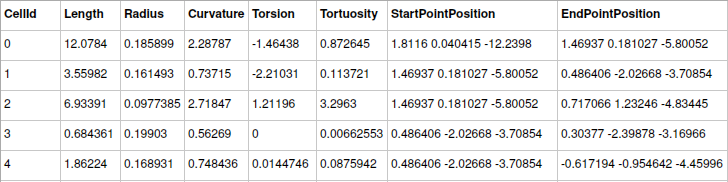
\includegraphics[width=\textwidth]{images/0053_extract4_cropped.png}
				\caption*{dimensions and connectivity}
				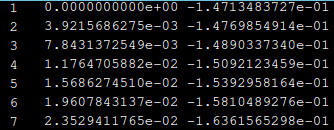
\includegraphics[width=\textwidth]{images/config0.png}
				\caption*{inflow data}
				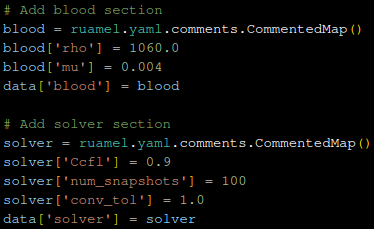
\includegraphics[width=\textwidth]{images/config1.png}
				\caption*{simulation constants}
			\end{figure}
	\end{minipage}}
	\onslide<2->{\begin{minipage}{0.1\textwidth}
			
\includegraphics[width=\textwidth]{images/right_arrow.png}
		\end{minipage}
		\begin{minipage}{0.25\textwidth}
			\begin{figure}
				\resizebox{\linewidth}{!}{\begin{minipage}{2.3\textwidth}
						\begin{align*}
							P_{mean} &:= \frac{120 \text{mmHg}}{80 \frac{\text{ml}}{\text{s}}}, \  Q_{car} := 80 \frac{\text{ml}}{\text{s}}, \\
							R_{tot} &:= \frac{P_{mean}}{Q_{car}}, \ C_{tot} := 10^{-3} \frac{\text{cm}^5}{\text{dyne}}, \\
							\gamma_i &:= \frac{\sum_{j \in I} A_{0,j}}{A_{0,i}}, \\
							R_{tot,i} &:= \gamma_i R_{tot}, \ C_{tot,i} := \frac{1}{\gamma_i} C_{tot}, \\
							R_{1,i} &:= \frac{9}{100} R_{tot,i}, \ R_{2,i} := \frac{91}{100} R_{tot,i}.
						\end{align*}
				\end{minipage}}
				\caption*{Windkessel parameters}
				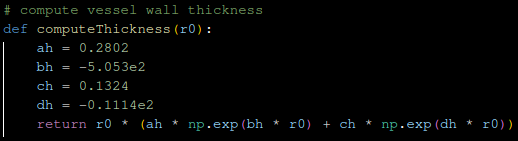
\includegraphics[width=\textwidth]{images/config2.png}
				\caption*{vessel wall thickness}
				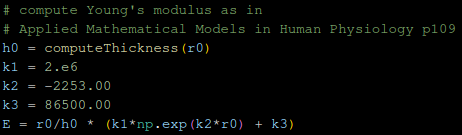
\includegraphics[width=\textwidth]{images/config3.png}
				\caption*{Young's modulus}
			\end{figure}
	\end{minipage}}
	\onslide<3->{\begin{minipage}{0.1\textwidth}
			
\includegraphics[width=\textwidth]{images/right_arrow.png}
		\end{minipage}
		\begin{minipage}{0.25\textwidth}
			\begin{figure}
				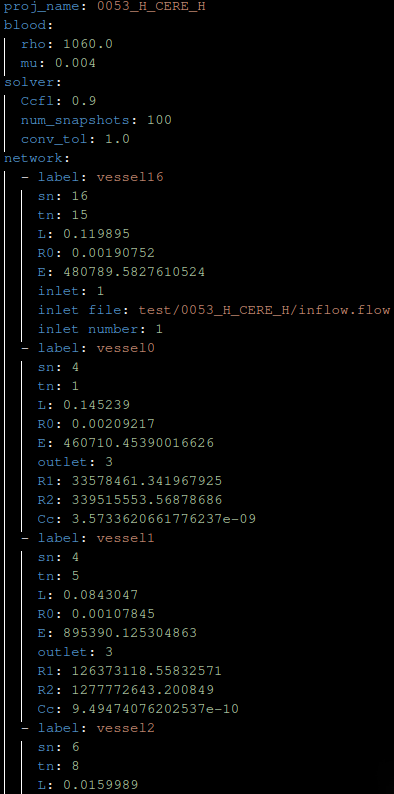
\includegraphics[width=\textwidth]{images/config4.png}
				\caption*{YML configuration}
			\end{figure}

	\end{minipage}}
\end{frame}

\subsection{Solver}
\againframe<7>{mp}

\begin{frame}
	\frametitle{Solver: Single Vessel (SV)}
	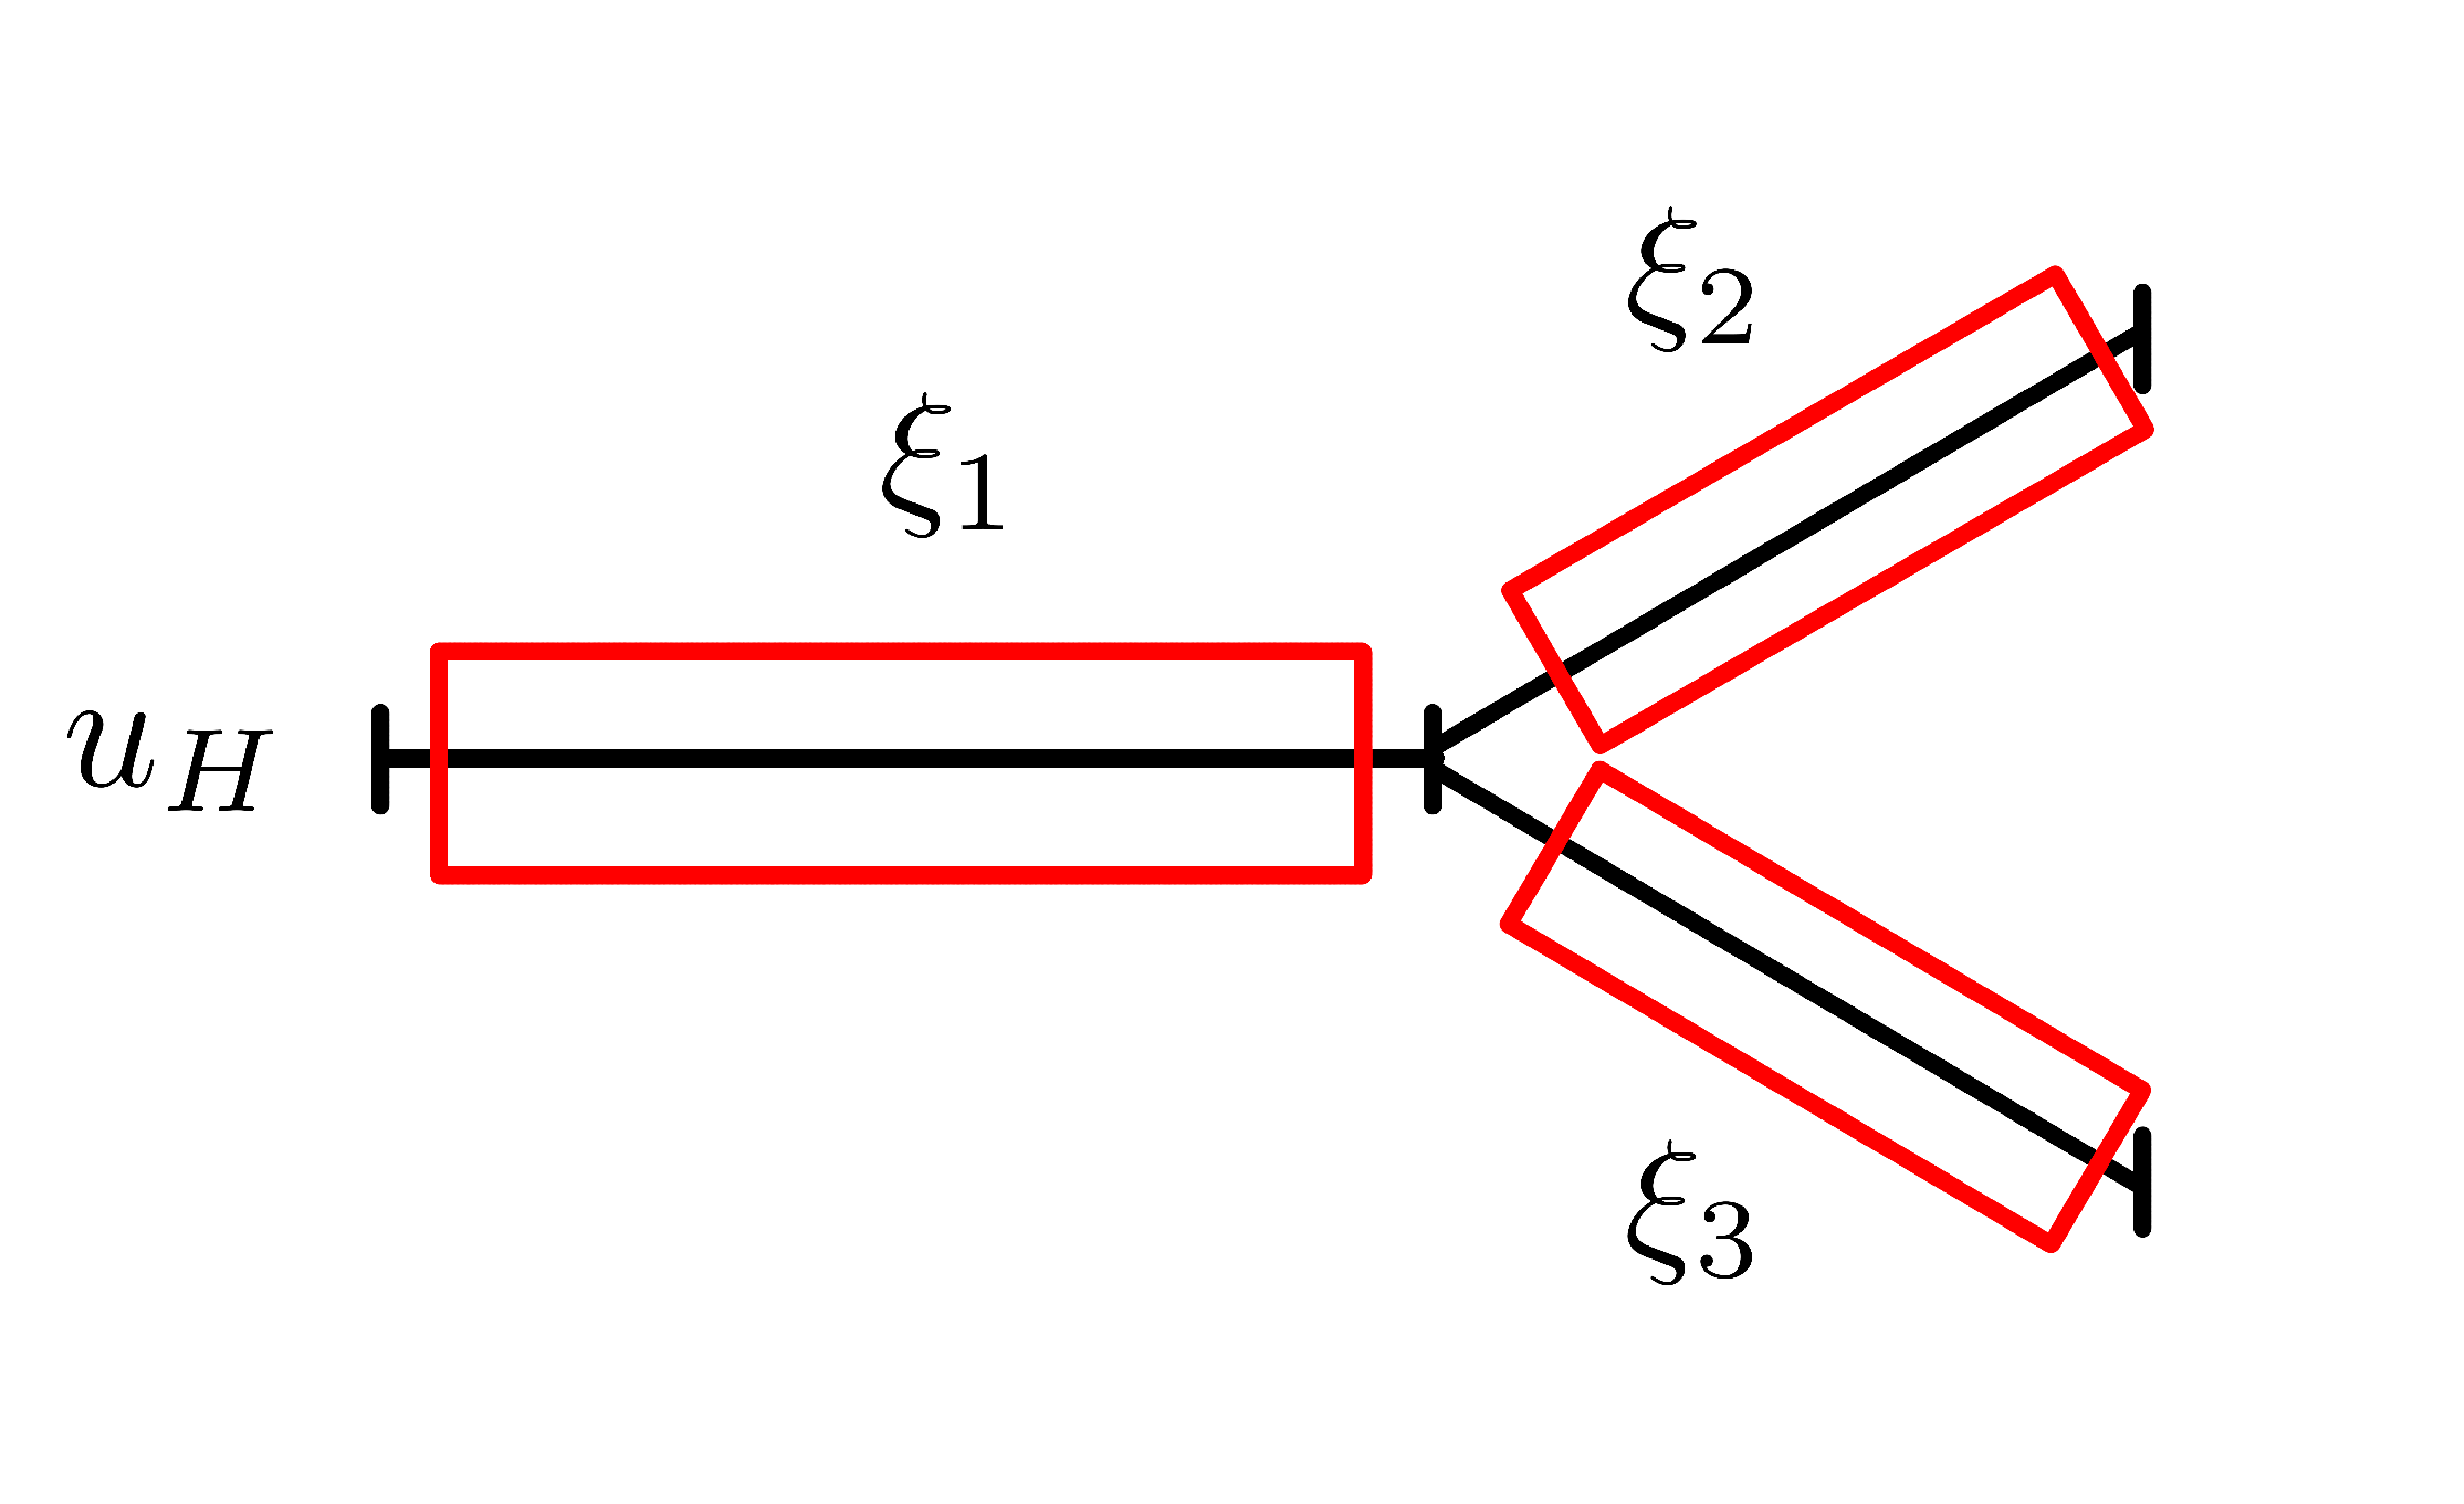
\includegraphics[width=\linewidth]{images/bifurcation_vessels.eps}
\end{frame}

\begin{frame}<1-4>[label=nse]
	\frametitle{Solver: 1D-Navier Stokes Equations (SV)}
	\begin{equation}
		\begin{aligned}
			\frac{\partial \mathbf{U}}{\partial t} + \frac{\partial \mathbf{F} \left(
			\mathbf{U} \right)}{\partial z} &= \mathbf{S} \left( \mathbf{U} \right), \ t>0, \
			z \in \left[ 0,l \right], \only<1>{\\
			\mathbf{U} \left( z;0 \right) &= \mathbf{U}_0 \left( z \right), \ z \in \left[ 0,l \right], \\
			\mathbf{U} \left( 0;t \right) &= \mathbf{U}_L \left( t \right), \ t>0,\\
		\mathbf{U} \left( l;t \right) &= \mathbf{U}_R \left( t \right), \ t>0,}
	\end{aligned} \label{eq:1deqs3}
\end{equation}
\begin{equation}
	\mathbf{U} :=
	\begin{bmatrix}
		A \\
		Q
	\end{bmatrix}, \ 
	\mathbf{F} \left( \mathbf{U} \right) :=
	\begin{bmatrix}
		Q \\
		\frac{Q^2}{A} + \frac{\beta A^{\frac{3}{2}}}{3\rho\sqrt{A_0}}
	\end{bmatrix}, \ 
	\mathbf{S} \left( \mathbf{U} \right) :=
	\begin{bmatrix}
		0 \\
		-22\frac{\mu}{\rho}\frac{Q}{A}
	\end{bmatrix}.
\end{equation}

\vfill

{\tiny \centering 
	\only<1>{$\mathbf{U_0} \hat{=}$ initial condition, 
		$\mathbf{U_L} \hat{=}$ left boundary values,
	$\mathbf{U_R} \hat{=}$ right boundary values,}

	$l \hat{=}$ vessel length,
	$A \hat{=}$ cross-section,
	$A_0 \hat{=}$ reference cross-section,
	$Q \hat{=}$ volumetric flow-rate,

	$\beta \hat{=}$ elasticity coefficient,
	$\rho \hat{=}$ blood density,
	$\mu \hat{=}$ blood dynamic viscosity. 
\par}

\only<2->{\vfill

	\begin{block}{Conservative Form with Source Term}
		\begin{itemize}
			\onslide<2->{\item conservation of mass (continuity equation)}
			\onslide<3->{\item conservation of momentum}
			\onslide<4->{\item no energy equation (incompressible Newtonian fluid)}
	\end{itemize}

\end{block}}



\end{frame}

\begin{frame}<1-2>[label=tl]
	\frametitle{Solver: Tube Law (SV)}
	\begin{align}
		P(z;t) &:= P_{ext}(z;t) + \beta \left( \sqrt{\frac{A(z;t)}{A_0(z)}}-1 \right),      \label{eq:p_tot}\\
		\beta(z) &:=  \frac{\sqrt{\pi} E h_0(z)}{(1-\nu^2) \sqrt{A_0(z)}},\  z \in \left[ 0,l \right], \ t > 0. 
	\end{align}

	\vfill

	{\tiny \centering 
		$P \hat{=}$ pressure,
		$P_{ext} \hat{=}$ external pressure,

		$l \hat{=}$ vessel length,
		$A \hat{=}$ cross-section,
		$A_0 \hat{=}$ reference cross-section,

		$E \hat{=}$ Young's modulus,
		$h_0 \hat{=}$ reference vessel wall thickness,
		$\nu \hat{=}$ Poisson's ratio (elasticity parameter). 
	\par}
	\onslide<1->{\begin{block}{Closure Equation}
			\begin{itemize}
				\onslide<1->{\item $P(z;t)$ describes pressure in relation to $A(z;t)$ }
				\onslide<2->{\item $\beta(z)$ quantifies structure}
		\end{itemize}
\end{block}}
\end{frame}

\begin{frame}<1-3>[label=ic]
	\frametitle{Solver: Initial Conditions (IC) (SV)}
	\onslide<1->{\begin{minipage}{0.37\textwidth}
			\begin{block}{Steady State}
				Since good IC are not known trivial ones are set and the simulation is run until a steady state is reached.
			\end{block}

	\end{minipage}}
	\hfill
	\onslide<3->{\begin{minipage}{0.57\textwidth}
			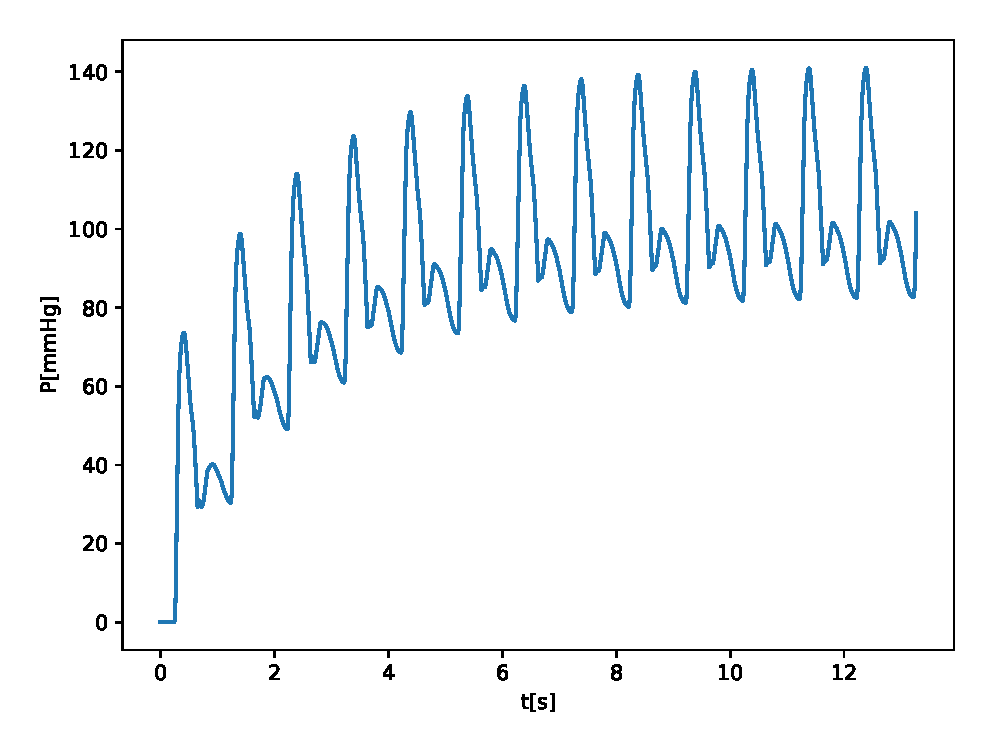
\includegraphics[width=\textwidth]{images/adan56_tibiofibular_trunk_L_P_steady_state.eps}
	\end{minipage}}
	\onslide<2->{\begin{align}
			u(z;0) &\equiv 0, &z \in [0,l],\\
			A(z;0) &= A_0(z), &z \in [0,l], \\
			Q(z;0) &= u(z;0)A(z;0) \equiv 0, &z \in [0,l].
	\end{align}}
\end{frame}

\begin{frame}
	\frametitle{Solver: Network (NW)}
	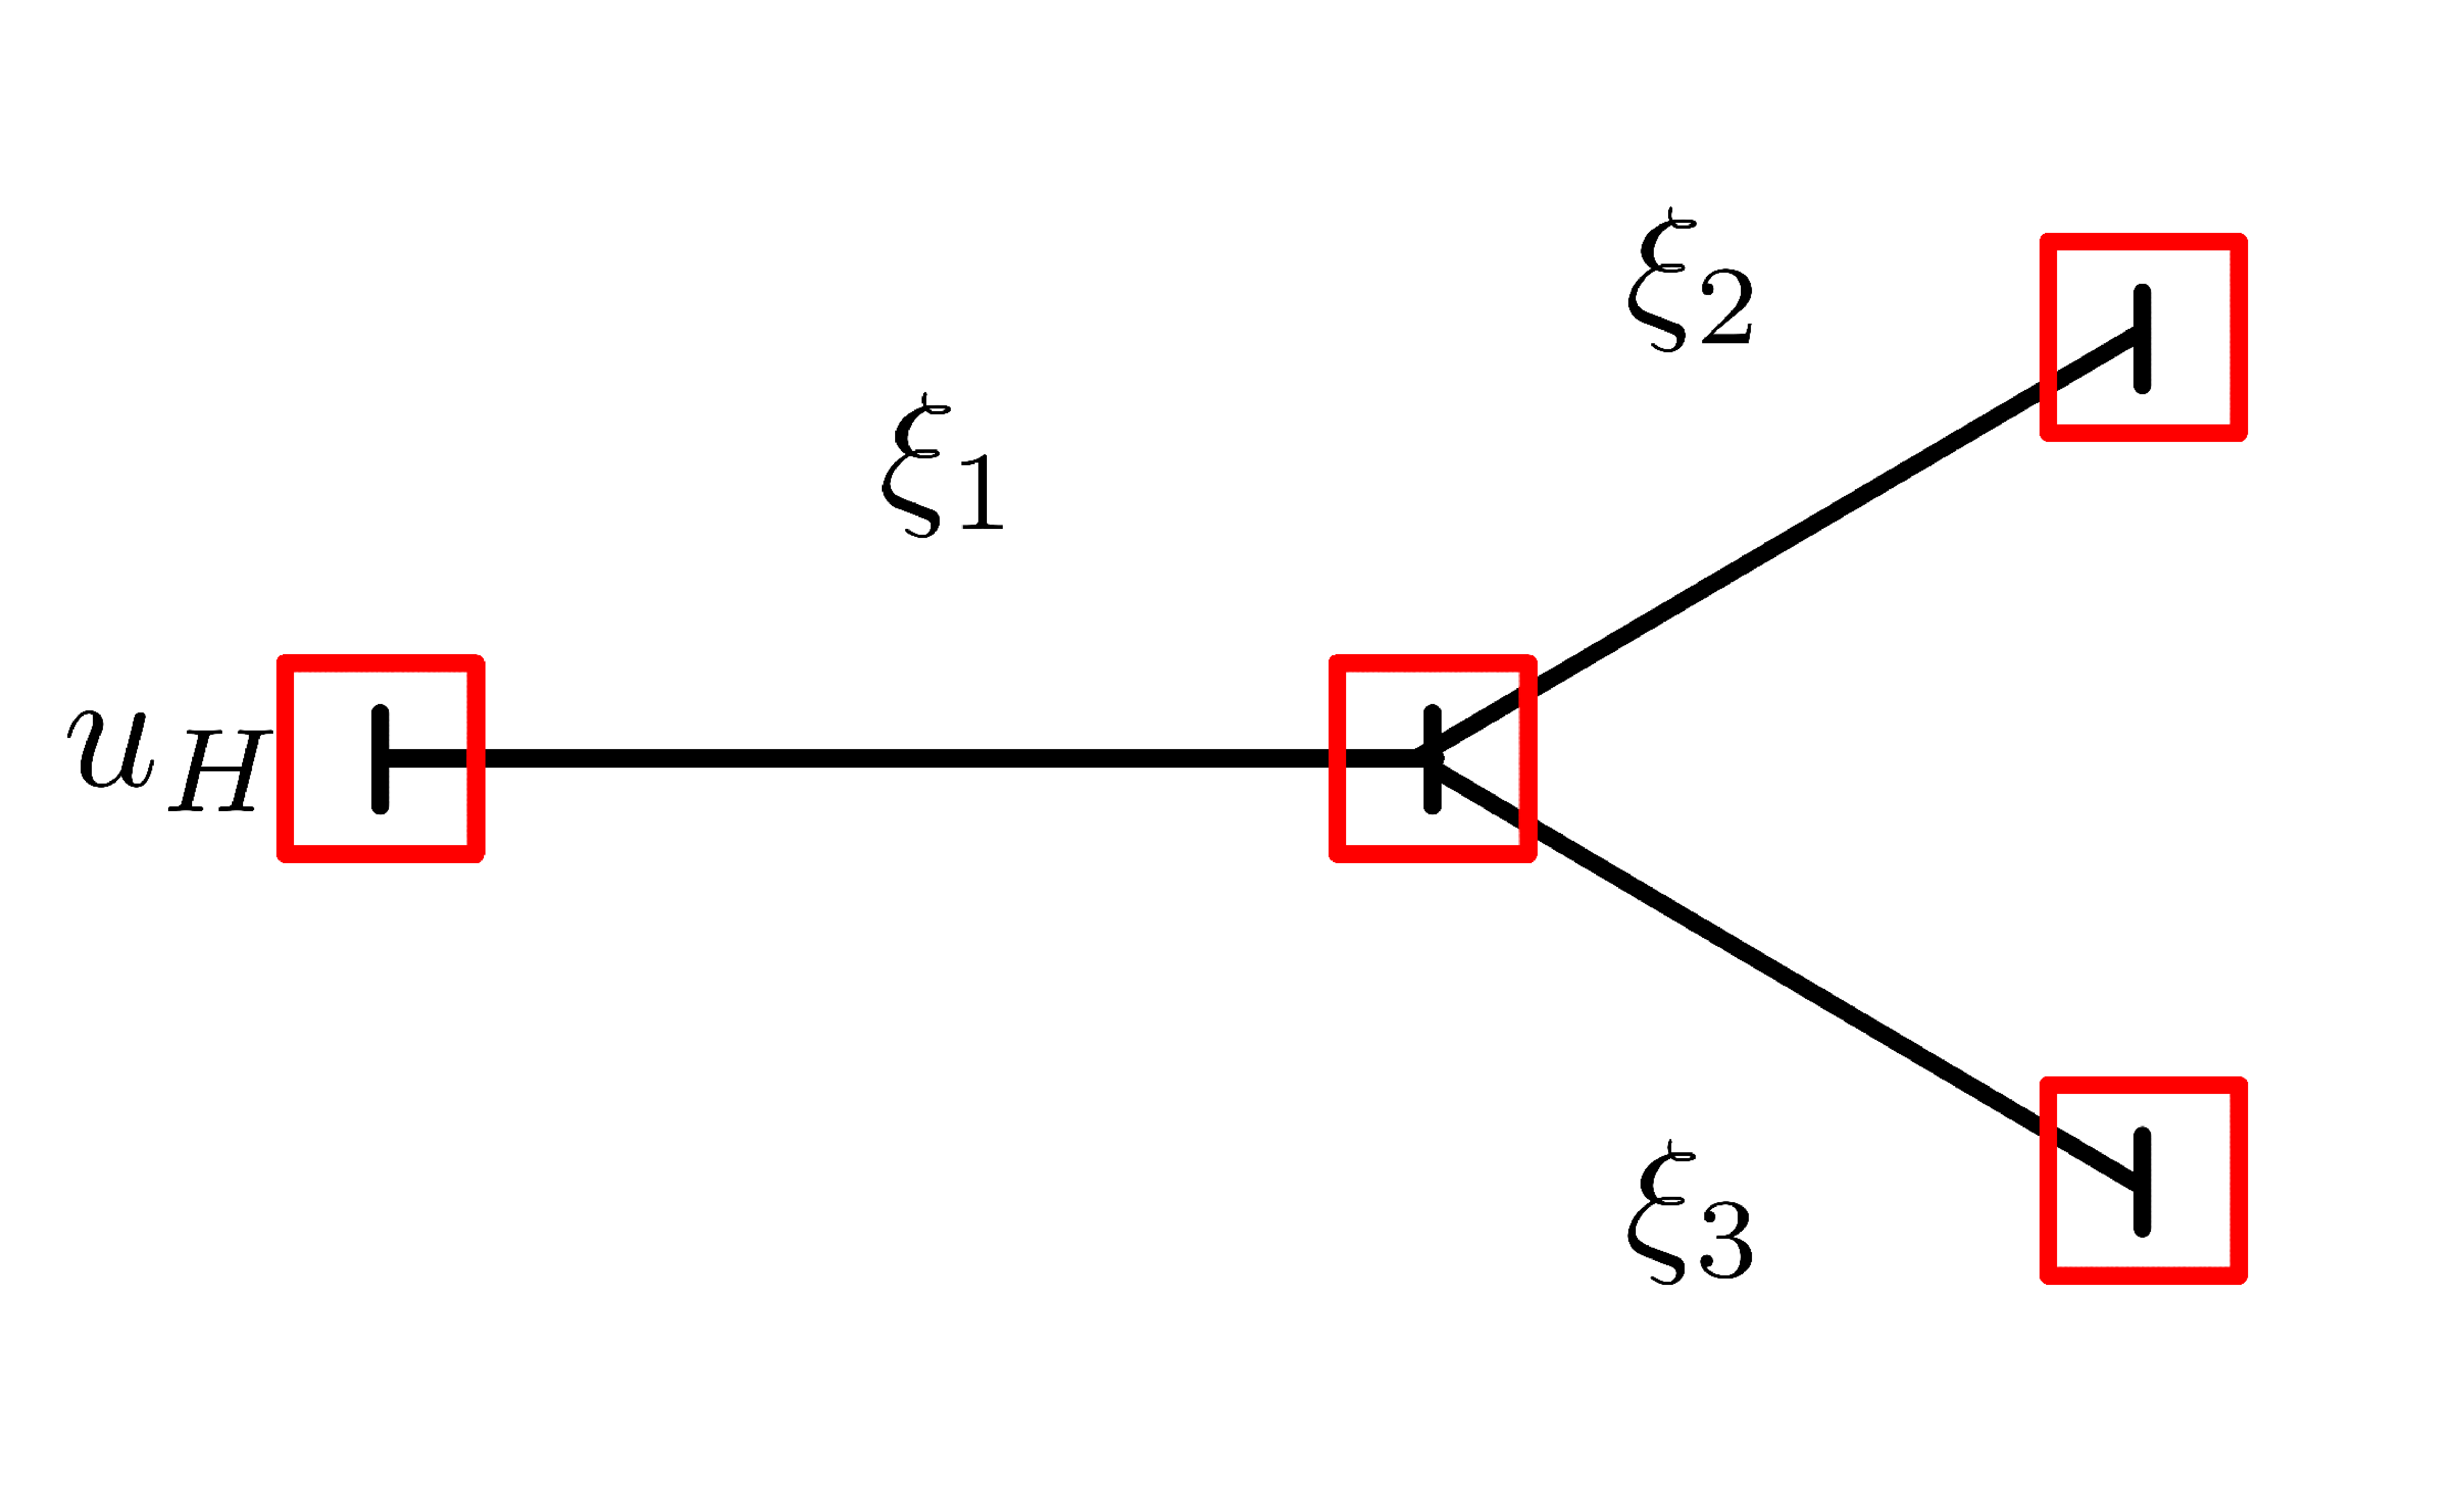
\includegraphics[width=\linewidth]{images/bifurcation_network.eps}
\end{frame}

\begin{frame}
	\frametitle{Solver: Inlets, Junctions, Outlets (NW)}
	\begin{block}{Inlets}
		\onslide<1->{set $P$ or $Q$ from data}
	\end{block}
	\begin{block}{Junctions}
		\onslide<2->{solve linear system of equations consisting of:
			\begin{itemize}
				\item conservation of mass and
				\item conservation of momentum.
		\end{itemize}}
	\end{block}
	\begin{block}{Outlets}
		\onslide<3->{0D-/ lumped parameter model: three element Windkessel (RCR) model}
	\end{block}
\end{frame}

\begin{frame}
	\frametitle{Solver: Numerical Methods (SV)\&(NW)}
	\begin{block}{1D-Model}
		\onslide<1->{Finite Volume (FV) method: monotonic upstream-centred scheme for conservation laws (MUSCL) with Lax-Friedrichs (LF) flux.}
		\begin{itemize}
			\onslide<2->{\item FV: for discrete domains and conservative equations}
			\onslide<3->{\item LF: for hyperbolic system}
	\end{itemize}
\end{block}
\begin{block}{Junctions \& Outlets}
	\onslide<4->{Newton method}
	\begin{itemize}
		\onslide<5->{\item for solving non-linear root finding problems}
\end{itemize}
\end{block}
\end{frame}

\begin{frame}
	\frametitle{Solver: JAX Caveats}
	\begin{block}{What to look out for:}
		\begin{itemize}
			\item<1-> functional purity
			\item<2-> efficient data structures
			\item<3-> avoiding for loops (loops in general)
				\begin{itemize}
					\item<4-> Python for-loop: \textcolor<5->{red}{slow compilation}
					\item<6-> JAX for-loop: \textcolor<7->{red}{homogeneous mesh }
					\item<8-> $\rightarrow$ \textcolor<9->{green}{ avoid for-loops through vectorization}
					\item<10-> $\rightarrow$ \textcolor<11->{red}{requires padding and masking}
				\end{itemize}
		\end{itemize}
	\end{block}
\end{frame}

\begin{frame}
	\frametitle{Solver: Padding}
	without padding
	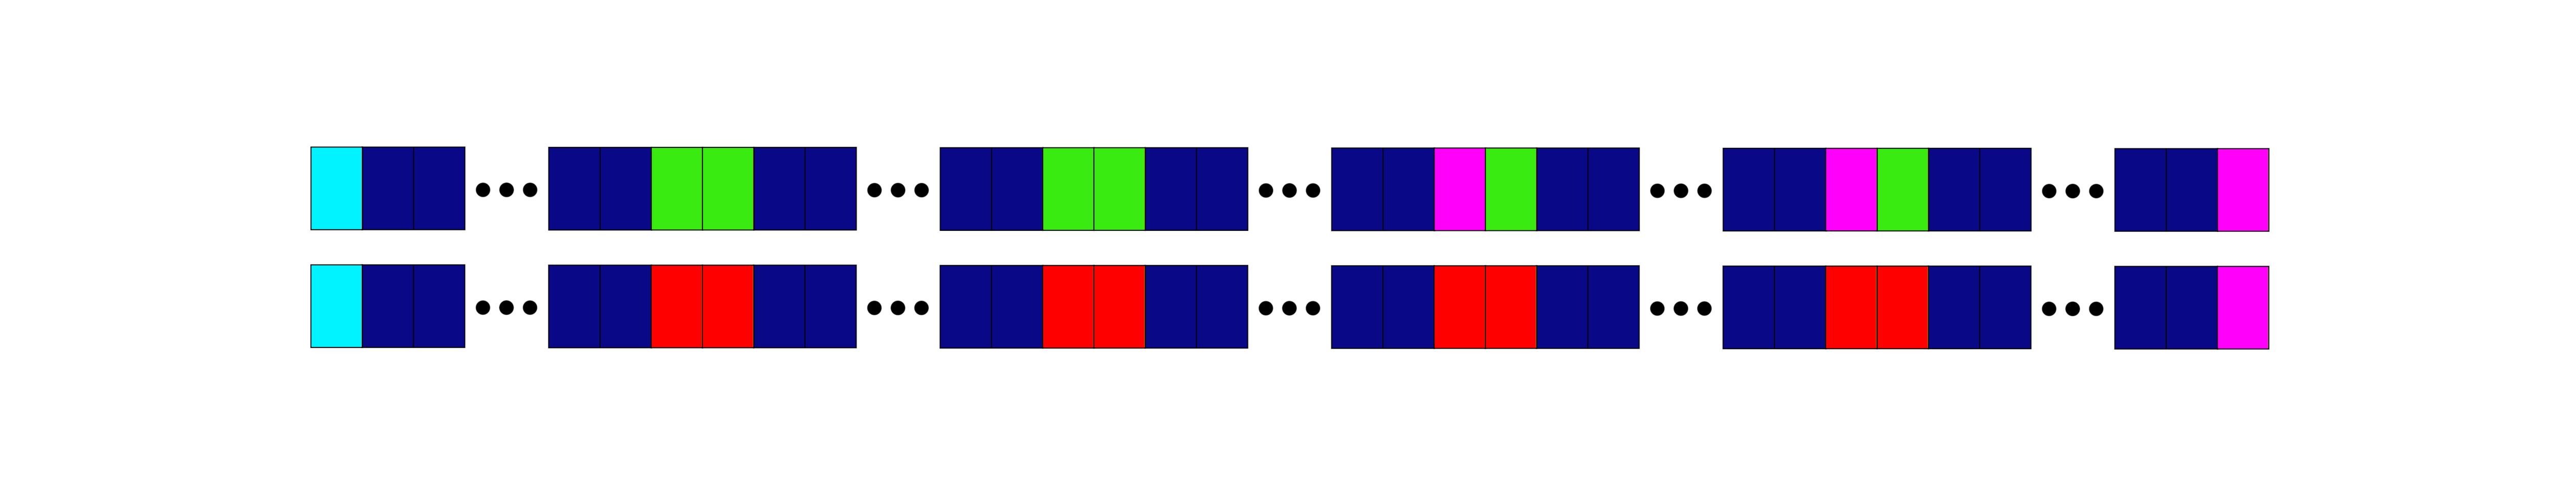
\includegraphics[width=\textwidth]{images/padding1.eps}
	with padding
	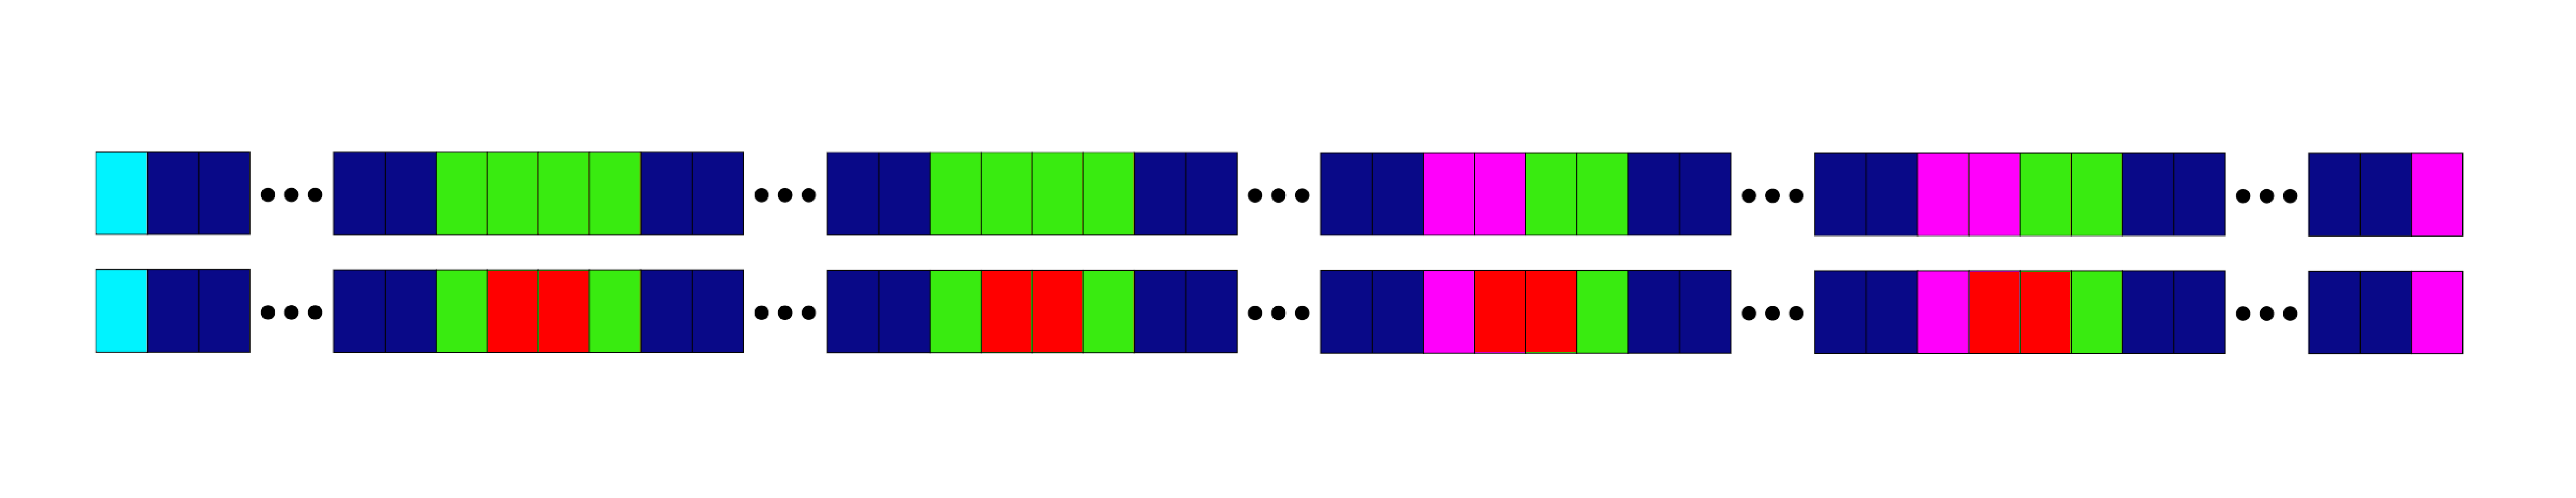
\includegraphics[width=\textwidth]{images/padding2.eps}
	\includegraphics[width=\textwidth]{images/legend.eps}
\end{frame}

\begin{frame}
	\frametitle{Solver: Masking}
	\includegraphics[width=\textwidth]{images/masking.eps}
	\includegraphics[width=\textwidth]{images/legend.eps}
\end{frame}

\section{Results}
\subsection{Biomarkers}
\againframe<8>{mp}
\subsection{Comparison}
\begin{frame}
	\frametitle{Comparison: Computed Biomarkers}
	\begin{figure} [H]
		\centering
		\includegraphics[width=0.46\columnwidth]{../figures/0007_H_AO_H_right_subclavian_artery_P.eps}
		\includegraphics[width=0.46\columnwidth]{../figures/0029_H_ABAO_H_celiac_branch_P.eps
		}
		\includegraphics[width=0.46\columnwidth]{../figures/0053_H_CERE_H_basilar_artery_IV_P.eps}
		\includegraphics[width=0.46\columnwidth]{../figures/adan56_common_hepatic_P.eps}
		\label{fig:val}
	\end{figure}
\end{frame}

\begin{frame}
	\frametitle{Comparison: Wall-clock Time}
	\begin{figure} [H]
		\centering
		\includegraphics[width=0.94\columnwidth]{../figures/timing_benchmark.eps}
		\label{fig:comparison}
	\end{figure}

\end{frame}

\subsection{Case Studies}
\begin{frame}
	\frametitle{Case Studies: Aorta (0007\_H\_AO\_H)}
	\begin{figure} [H]
		\centering
		\includegraphics[width=\columnwidth]{images/0007.eps}
		\label{fig:aorta}
	\end{figure}
\end{frame}
\begin{frame}
	\frametitle{Case Studies: Abdominal Arteries (0029\_H\_ABAO\_H)}
	\includegraphics[width=\columnwidth]{images/0029.eps}
\end{frame}
\begin{frame}
	\frametitle{Case Studies: Cerebellar Arteries (0053\_H\_CERE\_H)}
	\includegraphics[width=\columnwidth]{images/0053.eps}
\end{frame}
\begin{frame}
	\frametitle{Case Studies: ADAN56}
	\includegraphics[width=\textwidth]{images/adan56.eps}
\end{frame}

\section{Parameter Inference}
\subsection{1D Model Pipeline Recall}
\againframe<9>{mp}
\subsection{Parameter Inference Pipeline}
\againframe<100>{mp}
\subsection{Parameter Inference}
\againframe<101>{mp}

\begin{frame}
	\only<1>{\frametitle{Parameter Inference: Simulation Wrapper}}
	\only<2>{\frametitle{Parameter Inference: Custom Log-Likelihood}}
	\only<3->{\frametitle{Parameter Inference: Numpyro Model}}

	\only<1>{\includegraphics[width=\textwidth]{images/inference1.png}}
	\only<2>{\includegraphics[width=\textwidth]{images/inference2.png}}
	\only<3->{\includegraphics[width=\textwidth]{images/inference3.png}
		Real value: $R = 6.82 \times 10^7$
		\begin{itemize} 
			\item<4-> \# warmup steps: 10, \# sample steps: 100, $R_{init} = 10^8$ $\rightarrow$ estimated parameter: $7.67 \times 10^7$, relative error: $\sim 13\%$, wall-clock time: $\sim 22$ minutes
			\item<5-> \# warmup steps: 10, \# sample steps: 200, $R_{init} = 10^8$ $\rightarrow$ estimated parameter: $6.96 \times 10^7$, relative error: $\sim 2\%$, wall-clock time: $\sim 38$ minutes
		\end{itemize}
	}
\end{frame}


\section{Future Work}
\subsection{Future Work}
\begin{frame}
	\frametitle{Future Work}
	\begin{block}{Main Points of Interest}
		\begin{itemize}
			\item<1-> improving performance (general \& GPU optimization)
			\item<2-> automate geometry extraction
			\item<3-> generalize code for junctions involving $N$ vessels
			\item<4-> stable parameter inference
			\item<5-> sensitivity analysis (global and local)
		\end{itemize}
	\end{block}
	\vspace{5mm}
\end{frame}


\section{Questions}
\subsection{Questions}
\begin{frame}
	\frametitle{Questions?}
	Thank you for your attention!
\end{frame}

\end{document}
